
\chapter{绪论}

\section{背景概述}


\begin{figure}[!b]
%\setlength{\abovecaptionskip}{-0.1cm} 
%\setlength{\belowcaptionskip}{-0.45cm}
\centering
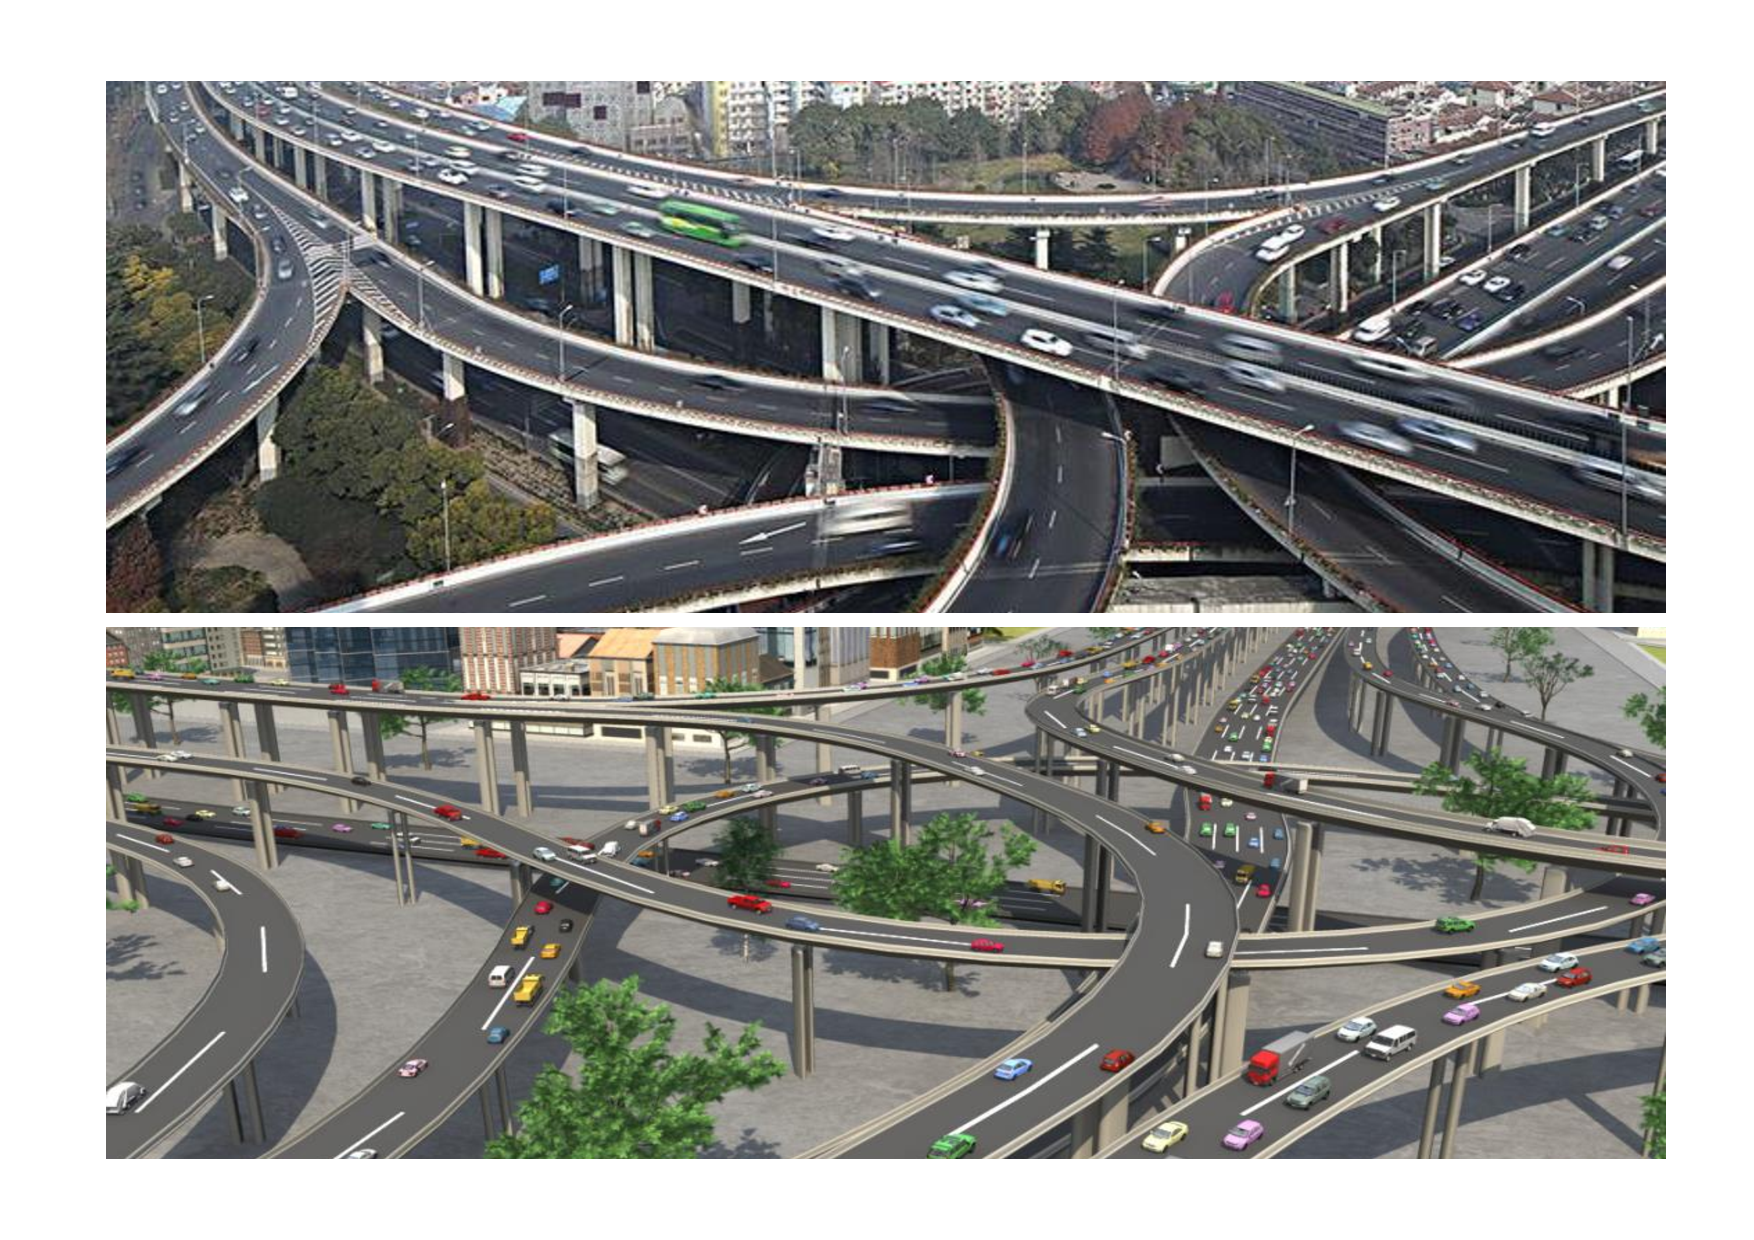
\includegraphics[width=\textwidth]{figure/intro/example.pdf}
%\caption[真实世界的交通与交通仿真结果]{
%真实世界的交通(上)与交通仿真结果~\cite{chao2017realistic}(下)。
%}
\caption[真实世界交通与交通仿真的可视化结果]{
真实世界交通(上)与交通仿真的可视化结果~\cite{chao2017realistic}(下)
}
\label{fig:intro_example}
\end{figure}

随着全球城市化进程的加速和人口的不断增长,大量车辆和行人在有限的道路空间内活动,随之出现的交通拥堵、交通事故、环境污染等问题对人类的生活和经济活动都产生了深远的影响,交通问题成为了当今社会面临的重要挑战之一。交通仿真作为计算机仿真领域的一个重要研究方向,通过设计模型和算法来模拟交通流动、道路网络、信号控制和交通规则,推演交通系统中车辆、行人和其他交通参与者的行为和交互过程。而随着计算机图形学和计算机视觉的进步,虚拟现实技术和三维动画与交通仿真得到了很好的结合,可视化交通仿真(visual traffic simulation)应运而生,其提供了逼真的可视化交通场景的同时,也帮助研究人员更好地理解交通行为和交通系统的性能。图~\ref{fig:intro_example}分别展示了真实世界的高架桥场景和高架桥可视化交通仿真的结果。利用交通仿真器,人们可以更好地理解和分析城市交通系统,以制定更有效的交通规划和管理策略,并进一步评估和测试这些新的交通设施、道路布局和管理策略的效果,以减少交通拥堵,提高交通流动性和安全性。


%此外,随着大数据、人工智能和云计算等领域的不断发展革新,涌现出了如自动驾驶、共享出行服务、数字孪生和智慧城市等新兴交通技术和出行模式。在这其中,自动驾驶作为备受青睐的热门技术,在提高交通安全和效率、提高人们出行体验、结合新能源推动可持续发展等方面被赋予了厚望。然而在自动驾驶技术在推广普及之前,仍然有许多艰巨的问题需要解决,

此外,随着新兴技术和出行模式的不断涌现,可视化交通仿真也被用于评估创新技术的性能和可行性,如自动驾驶技术、共享出行服务、数字孪生与智慧城市等。其中,自动驾驶在提高交通安全和效率、提高人们出行体验、结合新能源推动可持续发展等方面被寄予厚望。虽然自动驾驶技术正在不断被完善,但想要完全消除技术故障和错误是十分困难的,复杂的交通环境、传感器故障、通信不佳等问题都有可能对自动驾驶车辆的策略和操作产生不确定的影响,从而威胁乘客和其他交通参与者的安全。根据美国国家交通安全管理局(NHTSA)报告的数据,从2021年6月到2022年5月,美国涉及自动辅助驾驶的汽车碰撞事故共计392起,其中特斯拉273起,本田汽车90起。可视化交通仿真作为自动驾驶重要的支持工具,不仅可以生成多样的仿真数据对算法训练使用的数据集进行增广,还可以创造一个足够真实的虚拟环境供自动驾驶车辆进行道路测试,在无需考虑安全和成本的情况下验证自动驾驶算法在面对复杂、极端情况下的鲁棒性,提前排查可能发生的危险。

在交通仿真技术发展的初期,研究的重心主要集中在交通流模型的开发和应用,这一时期的模型大多基于流体动力学的理论,主要以交通流量、速度和密度等参数作为研究对象。近年来,由于人工智能技术的快速发展,交通仿真也迎来了新一轮革新,许多基于深度学习的交通仿真模型被开发出来,从采集到的数据中学习隐含的驾驶员决策和行为。然而,目前的交通仿真方法几乎都倾向于仿真平稳的车流,包括常见的加减速、变道、跟随前车、信号灯控制以及数据集中采集到的其他行为。而有些非常规的数据则容易被忽视,比如数据集中较少出现但现实生活中仍然有可能发生的车辆运动。因此,假设用户想要使用交通仿真器生成一些非常规的、带有特定车辆行为的交通数据,则需要根据前一次结果对仿真器的参数或者场景的预设进行调整并重新仿真,在结果仍然不理想时还要反复进行这一调试,直到最终的结果符合用户预期为止,这是一个十分繁琐的试错过程。为了解决相似的问题,在群组动画的另一个领域——人群动画中,研究者们引入交互式编辑技术,提出了可以运用基于几何变形或绘制草稿线等方式去实时控制和引导人群运动的行为细节~\cite{kim2014interactive, montana2017sketching},如图~\ref{fig:intro_intercrowd}所示。但人的运动拥有更高的自由度,例如可以在某一时刻随意改变朝向,也可以像螃蟹一样横向运动;而车辆则必须严格按照其运动学模型和交规约束运动,否则会大大降低仿真结果的真实性和生成数据的可靠性。因此,如何将交互式编辑技术引入可视化交通仿真中,在保证仿真行为真实性和运行效率的同时,提高用户定制化生成的效率和仿真行为的多样性是本文的主要出发点之一。


\begin{figure}[!tbh]
\centering
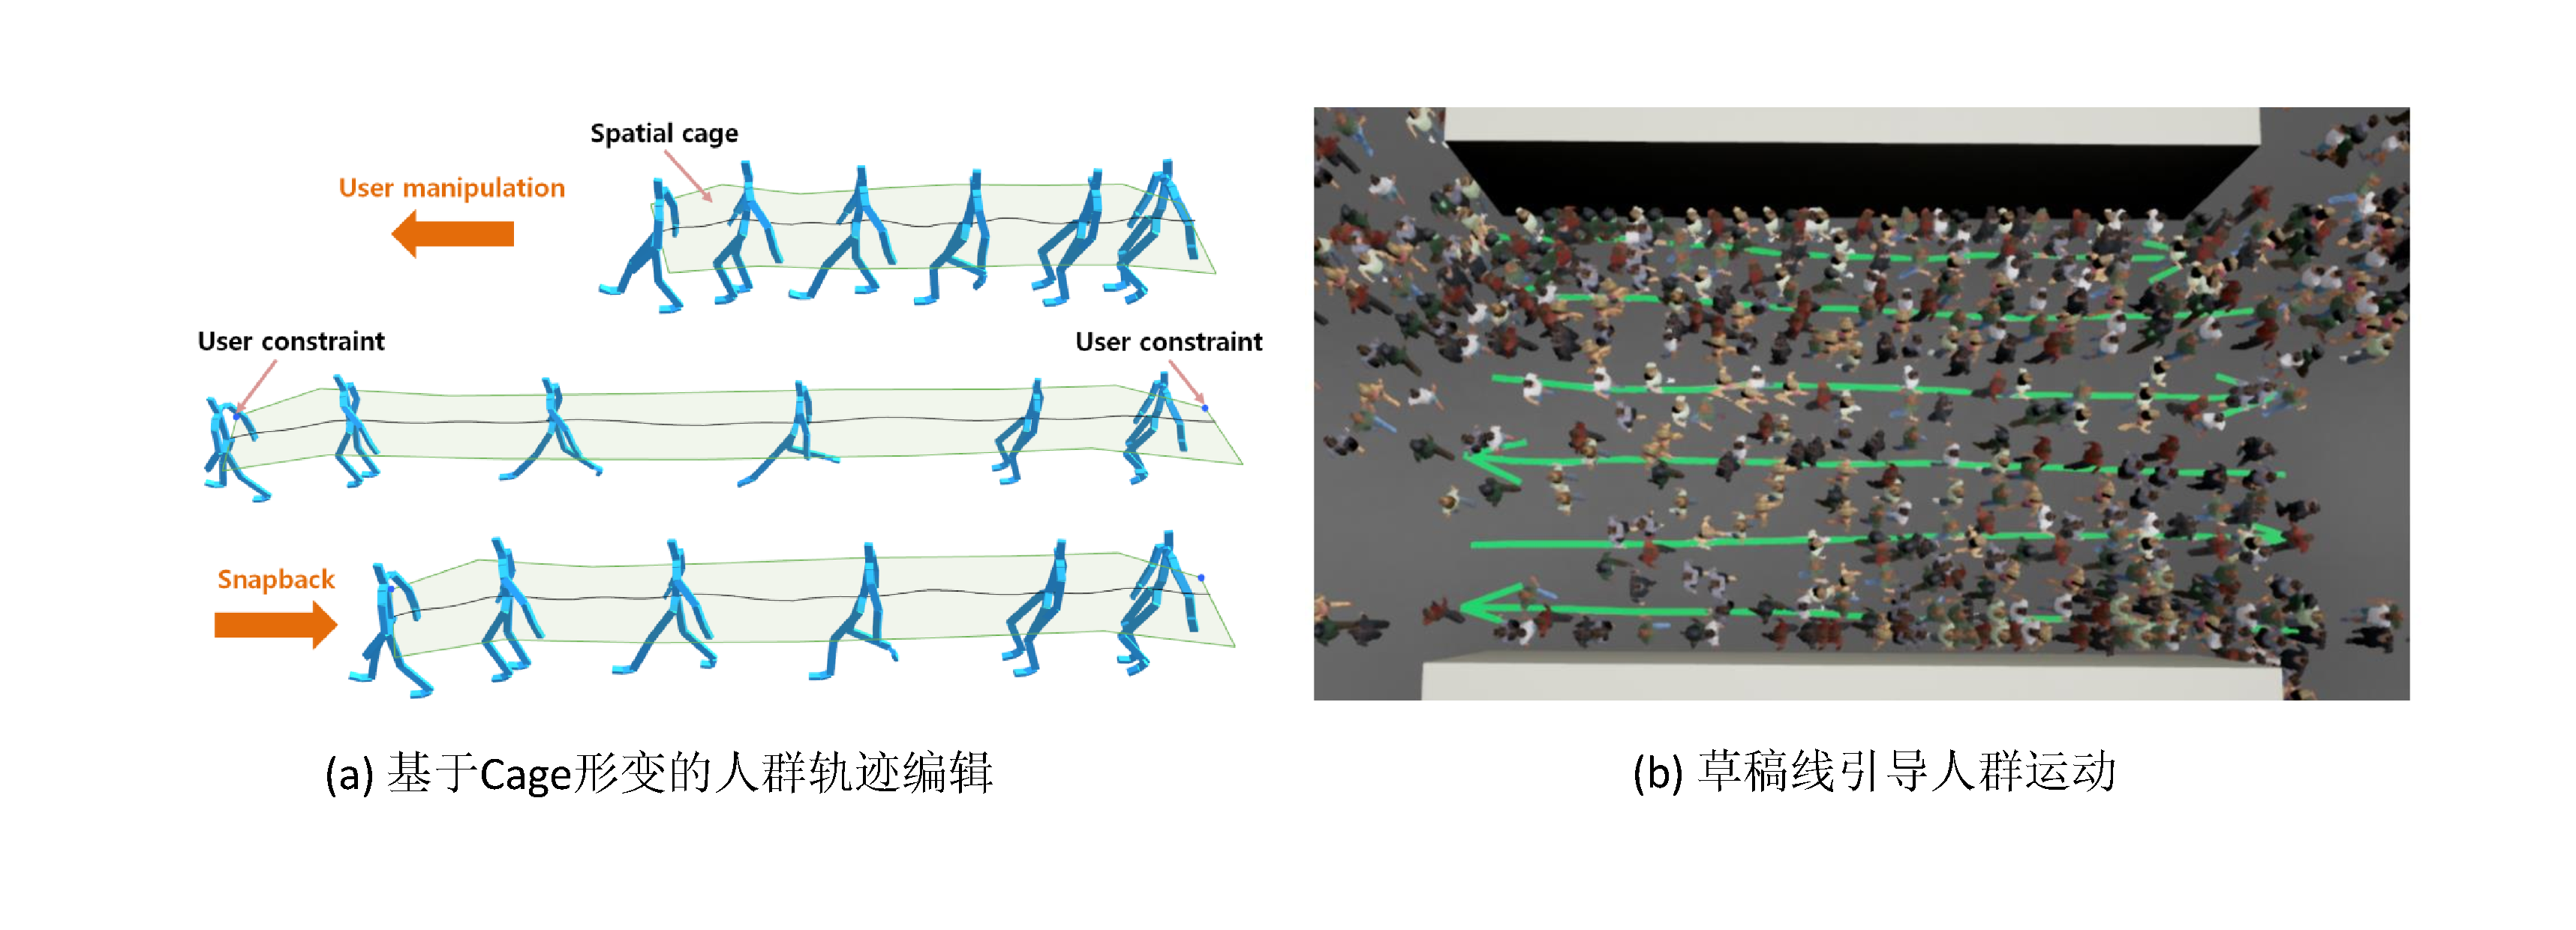
\includegraphics[width=\textwidth]{figure/intro/crowd interactive v2.pdf}
%\caption[人群动画交互式编辑]{
%(a) 基于cage形变的人群轨迹编辑~\cite{kim2014interactive}。(b) 使用草稿线引导人群运动~\cite{montana2017sketching}。
%}
\caption[人群动画中的交互式编辑技术]{
人群动画中的交互式编辑技术
}
\label{fig:intro_intercrowd}
\end{figure}

%在本章接下来的内容中,我们将介绍相关领域的研究背景和现状:首先我们会针对交通仿真所使用的各类模型依次进行简单的回顾,然后对车辆运动所使用的运动学模型、状态表示以及运动控制方法进行详细的介绍,接着对目前交互式编辑技术流行的应用领域和编辑方式分别进行介绍,最后明晰本文的主要研究内容和后续的行文结构。

%在本章接下来的小节中,将详细介绍各个领域的研究现状:首先我们将介绍群组动画和交通仿真的发展融合与现阶段的应用和挑战,然后本文会针对群组动画中的运动控制技术进行回顾,接着介绍交通仿真中所使用的车辆运动学建模和驱动模型类型,最后对目前交互式编辑技术流行的应用领域和编辑方式分别进行介绍。在介绍了相关技术的研究现状后,我们也会明晰本文的主要研究内容和后续的行文结构。另外,为了叙述简洁考虑,本文后续涉及到的交通仿真的部分,若无特殊及时,均指代可视化交通仿真技术。



\section{可视化交通仿真}


\subsection{群组动画与交通仿真的融合}

近年来,随着计算机硬件发展和软件算法的进步,计算机动画和虚拟现实技术开始得到广泛的应用,从电影、游戏到各种模拟和仿真都开始在三维场景中进行可视化来增加结果呈现的真实感和沉浸感。与此同时,在交通领域,由于问题的复杂性和多变性,简单的数学模型和统计数据已经无法满足决策者和公众日益增长的需求,研究者开始探索如何将交通仿真与计算机图形学相结合,提供更为直观和真实的交通情况展示。这种融合使得交通工程师、城市规划者和决策者可以更加直观地了解交通流量、拥堵情况、驾驶行为等问题~\cite{wang2017survey}。因此,可视化交通仿真(visual traffic simulation)应运而生,这是一项融合了场景路网建模~\cite{chen2008interactive, bruneton2008real, galin2010procedural, galin2011authoring}、汽车运动行为建模~\cite{reynolds1999steering, reynolds1987flocks}、场景动画的渲染绘制~\cite{tecchia2002image, o2002levels}和其他物理特效模拟等多个课题的技术。

本质上来说,由于车辆通过人的驾驶行为来控制,汽车的运动便可以看做是由人驾驶的智能体的运动,因此可视化交通仿真也可以作为群组动画的一种特殊类型,借鉴群体动画中运动控制的思路(章节~\ref{section:intro_crowdcontrol}),并融合车辆特定的行为约束(章节~\ref{section:intro_vehiclemove})来展开研究。最终,在一个由人、车、路、环境和交规等多因素构成的复杂交通网络系统中,各个智能体依据策略进行互动互融,呈现出多行为主体、自组织性、积累效应、框架效应等特征的模拟~\cite{brockmann2006scaling, barabasi1999emergence, dianhai2001traffic}。而将高细节、高逼真度的建模与动画与仿真结果相结合,可以大幅度提高展示结果的可信度和增强视觉体验,生成的多维度数据也可以进一步用于辅助指导交通设计、城市规划和自动驾驶训练测试等领域。


\subsection{应用场景示例}
\label{section:intro_apply}

首先,在传统的影视和游戏领域中,为了逼真再现虚拟环境中的城市场景、提升体验者的沉浸感,在建筑物、街道等静态环境中填充可视化的动态交通流是行之有效的方法之一,例如虚拟城市仿真软件Virtual Earth、CityEngine和City Life等~\cite{wang2017survey},以及一些高热度游戏如侠盗猎车手5和赛博朋克2077(游戏截图如~\ref{fig:intro_games}所示)。与影视特效中不计时间成本的离线仿真过程不同,游戏中填充的车流在没有玩家高度干预时,整体运行上更倾向于是平稳、协调且无碰撞的,这通常是制作人在考虑了游戏的实时性能需求、还原现实、强调用户操作与非用户操作之间的体验对比、设计美学等等多方面因素之后的结果。

\begin{figure}[!tbh]
%\setlength{\abovecaptionskip}{-0.1cm} 
%\setlength{\belowcaptionskip}{-0.45cm}
\centering
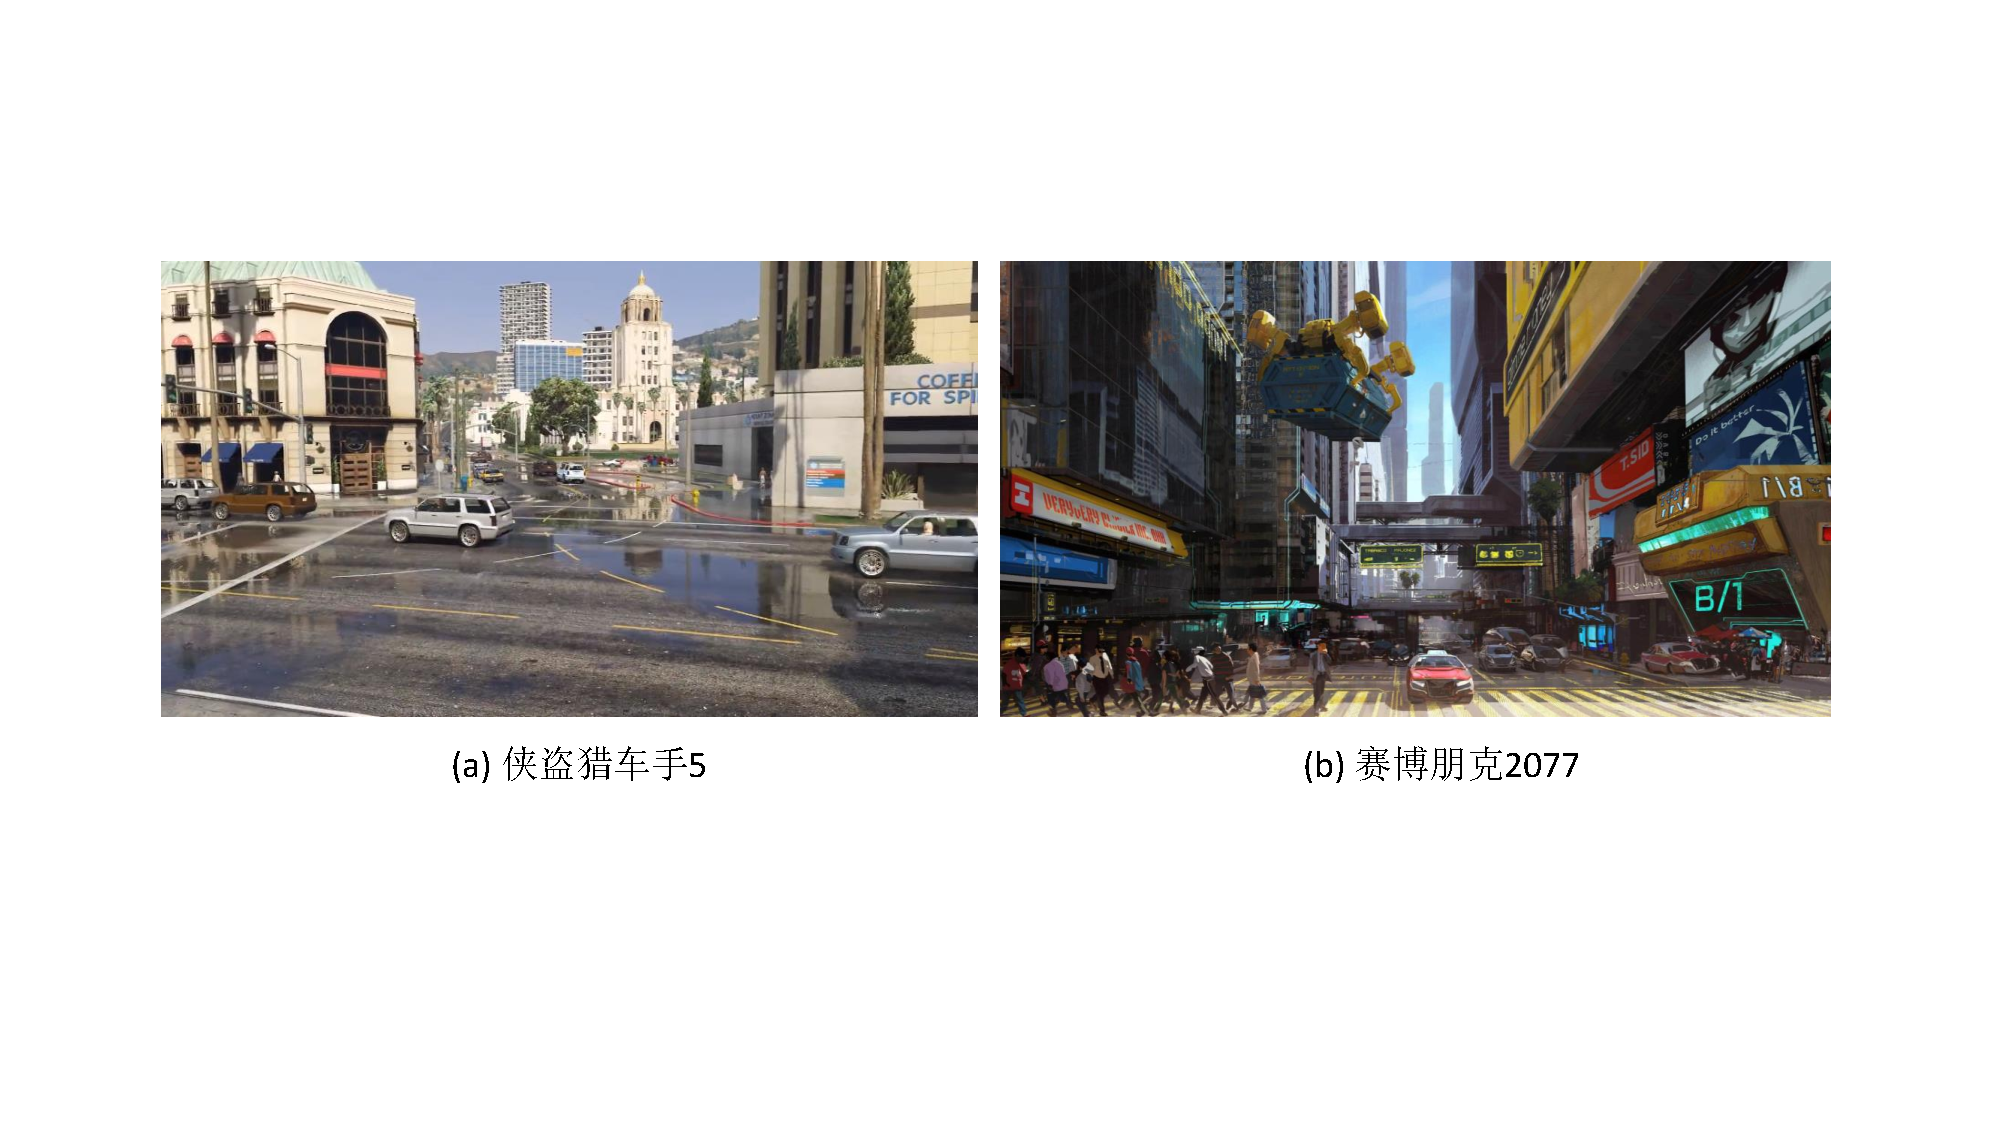
\includegraphics[width=\textwidth]{figure/intro/games.pdf}
%\caption[真实世界的交通与交通仿真结果]{
%真实世界的交通(上)与交通仿真结果~\cite{chao2017realistic}(下)。
%}
\caption[游戏场景中的可视化交通仿真车流]{
游戏场景中的可视化交通仿真车流
}
\label{fig:intro_games}
\end{figure}

%其次,自动驾驶作为近几年来交通仿真的一个重要下游应用,大量使用了可视化交通仿真技术来获取虚拟仿真数据,或是通过构建尽可能接近真实世界的三维系统来一定程度上取代实车的路测,这是传统基于数学和统计的交通仿真算法无法实现的。其主要目的有三个:
其次,自动驾驶作为近几年来交通仿真一个新兴而重要的下游应用,大量使用了可视化交通仿真技术来获取增广数据,或是通过构建尽可能接近真实世界的三维系统来一定程度上取代实车的路测。这在自动驾驶领域被称为World-Sim~\cite{hu2023ir, wang2023interpretable},即将自动驾驶算法控制的车辆(ego-car)置于实时仿真算法生成的车流中,其主要目的有三个:
\begin{itemize}
    \item 降低自动驾驶系统测试和回归的时间与成本;
    \item 实现各种边缘案例的人工构造,从而提升道路测试的覆盖面;
    \item 避免实车路测带来的人身财产安全损失和违法违规风险。
\end{itemize}
其中,边缘案例(corner case)特指发生概率低、数据集中可能会被遗漏的场景。与World-Sim相对应的是Log-Sim,是指通过在实际道路采集行驶各类记录(如自车和周车的位置速度信息、行车视频等),通过平台回放来实现场景的再现~\cite{hu2023ir, wang2023interpretable}。虽然Log-Sim能保证数据是真实无误的,但其内容无法根据不同的测试需求进行更改,回放中的周车对自车的行为变化也无法再做进一步的反馈,因此Log-Sim并非真正意义上的仿真。以Carla仿真平台~\cite{dosovitskiy2017carla}为例,其为自动驾驶的训练和测试提供了丰富的多维度信息,包括逼真的城市环境、不同的天气条件、模拟各类传感器(如摄像头、雷达和激光雷达)以及为视觉任务提供准确的真值(ground truth)等等,这得益于虚拟世界中所有物体的几何、位置信息都是提前已知的。如图~\ref{fig:intro_application}(a)所示是Carla官方提供的ego-car在可视化交通仿真车流中的行车视频,以及对应的语义分割结果;图~\ref{fig:intro_application}(b)则是通过混合现实技术,在真实采集的行车视频中重建三维场景并填充、渲染逼真的仿真交通流~\cite{li2019aads}用于数据增强。

%如图~\ref{fig:intro_application}所示是Carla官方提供的ego-car在可视化交通仿真中模拟行车视频的某一帧截图,以及其对应准确的深度检测和语义分割结果。这些信息既可以用于检验用户提出的图片处理算法的鲁棒性,也可以直接作为自动驾驶算法的输入用于自车控制的训练和测试。

\begin{figure}[!tbh]
%\setlength{\abovecaptionskip}{-0.1cm} 
%\setlength{\belowcaptionskip}{-0.45cm}
\centering
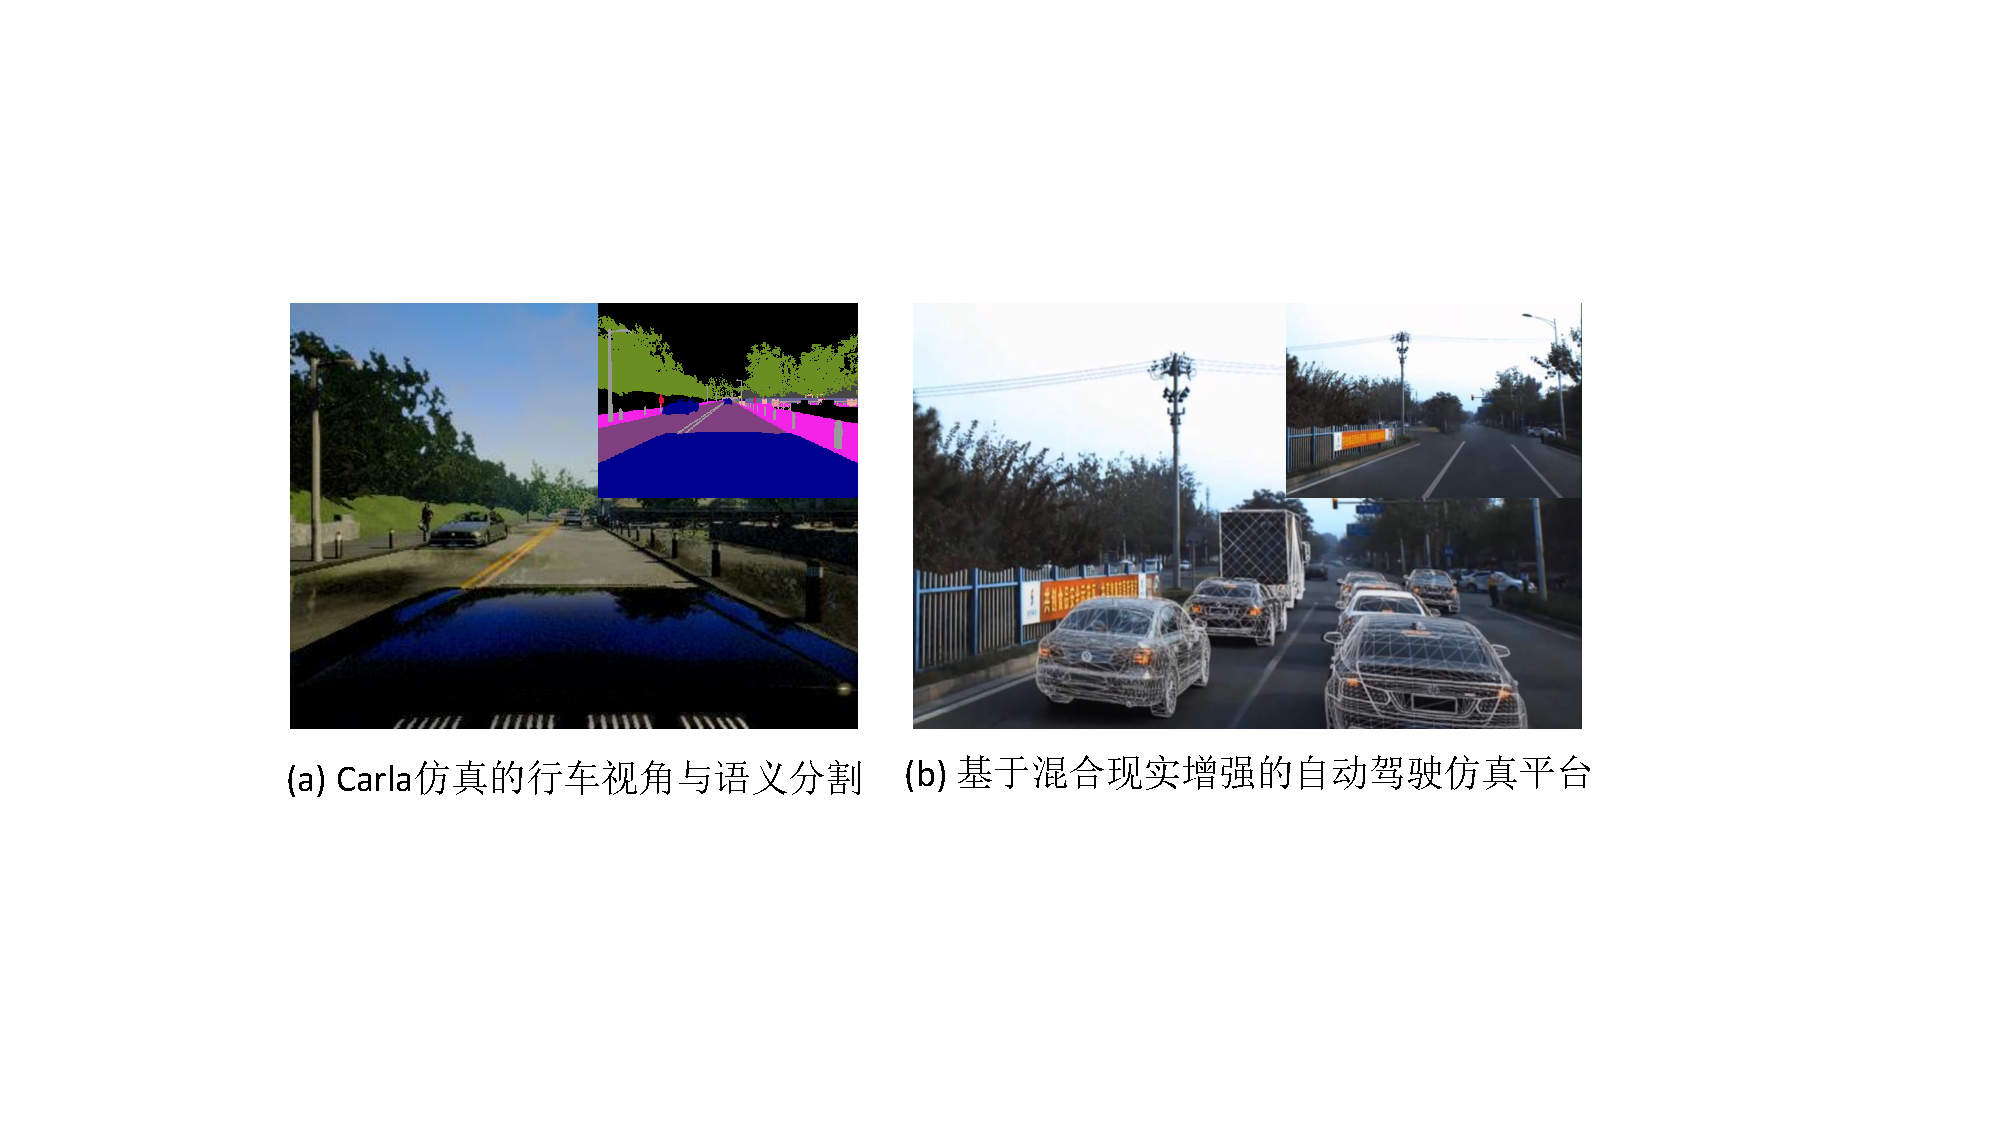
\includegraphics[width=0.85\textwidth]{figure/intro/application.pdf}
%\caption[真实世界的交通与交通仿真结果]{
%真实世界的交通(上)与交通仿真结果~\cite{chao2017realistic}(下)。
%}
\caption[自动驾驶中的可视化交通仿真]{
自动驾驶中的可视化交通仿真
}
\label{fig:intro_application}
\end{figure}



\subsection{可视化交通仿真面临的挑战}
\label{section:intro_challenge}

虽然可视化交通仿真在众多应用中已经取得了显著的成绩,但是对于日益复杂庞大的交通环境和不断增长的用户需求,除了已经能模拟的常见交通行为(如加减速、简单变道、跟随前车等)之外,如何高效快捷地生成更多样化的交通行为是困难的,一般来自以下几个方面的挑战:

\begin{itemize}
    \item \textbf{行为真实性与多样性相互制衡:}可视化交通仿真更加注重道路级别(lane-level)的运动行为模拟,即微观级别的仿真,这是因为相比于传统的交通仿真其在视觉呈现上有着更高的要求。例如在经典的SUMO交通仿真软件~\cite{krajzewicz2002sumo}中,一些变道决策会直接让车辆从现车道瞬移到目标车道,若直接进行三维可视化呈现,则会大大降低构建的城市交通场景的真实程度。因此可视化交通仿真中所有的车辆都要保证轨迹足够平滑、精细,不会出现任何失真的大尺度状态跳变(如速度、方向、位置等)。受限于真实感要求,现有的可视化交通仿真方法仍倾向于保守地生成常规的车辆运动,因为将非常规驾驶行为直接集成到运动控制策略中,不仅难以对行为发生诸多影响因素建模(如心理、生理、社交、环境等),还会增加仿真中个体交互的复杂程度,间接提高了运动失真的风险;但若能鲁棒地在平稳车流中引入部分非常规的行为,其实又能提高最终仿真结果整体的视觉观感。所以,既能保证行为真实又能提高其多样性的运动控制方法是一个具有挑战的问题。


    %可视化交通仿真除了要处理大量交通仿真中的动态交互,还需要实时渲染大量的复杂对象,例如考虑天气、光照、阴影、反射等效果,这对方法整体的计算性能提出了很高的要求——如果在交通仿真为每一个仿真个体消耗大量时间用于路径规划、决策制定或者交互影响的计算,势必会牺牲渲染质量以保证实时效率。
    \item \textbf{计算性能制约模型复杂度:}研究者们尝试过为每一个仿真个体均使用完备的实时路径规划、决策制定或者交互影响计算(如几何级别的碰撞检测等),这样的策略确实能在保证行为真实的情况下引入更复杂的运动,但是同时也会限制仿真群体的规模、牺牲呈现结果的质量和降低用户的体验。正如~\ref{section:intro_apply}中所列举的很多应用场景都对可视化交通仿真方法整体的性能提出了很高的要求(自动驾驶World-Sim获取大量测试边缘案例、游戏实时反馈等),因为除了要处理大量仿真中的动态交互,还需要实时渲染大量的复杂对象(如建筑、道路、车辆、行人等)以及天气、光照、阴影和反射等特效以提高视觉真实感。所以,简单地为每一个个体引入更精细运动控制而牺牲计算效率、延长用户等待并不可取。


    \item \textbf{用户交互体验亟待提高:}为了让用户能够更好地理解和获取仿真结果,需要更加丰富的交互功能。虽然目前的可视化交通仿真方法中已有能支持如视角缩放旋转、对象选择、修改部分参数等操作,但仍然缺少对个体运动的深度干预,即:用户在开始仿真之后便难以对个体的行为细节进行把控,只能仍由其随既定的驱动策略运动发展,导致最终的仿真结果随机性非常大。假设用户要获得定制化的结果,则需要基于前一次结果去反复调试仿真参数和三维场景的预设,非常的繁琐。而从引入非常规驾驶行为的角度来说,倘若用户可以实时对仿真中的个体进行多维度的控制,便可以将驾驶员的心理、生理、社会和环境因素从个体运动控制策略中弱化,巧妙地将仿真个体非常规的决策过程转化为用户监督过程。遗憾的是,虽然提供流畅且直观的交互方式可以借助用户引导来提高仿真行为多样性、改善用户获取定制化数据的效率,但目前仍然缺少相关的技术支撑,如何设计用户的交互逻辑并与仿真中的运动控制方法相结合也是一个迫切需要解决的问题。

\end{itemize}



\section{本文内容及结构}


%本文的章节将在回顾相关工作之后,详细介绍我们提出的交通仿真与其交互式编辑技术,基于简化社会力模型的混合交通仿真、非常规性与多样性注入的实时交通轨迹编辑、由粗到细求解时-空关键帧约束的交通仿真以及引入非跟驰车辆行为的交互式交通仿真,各工作之间的关系如图~\ref{fig:intro_overview}。本文后续的内容安排如下:

%\begin{figure}[!tbh]
%\centering
%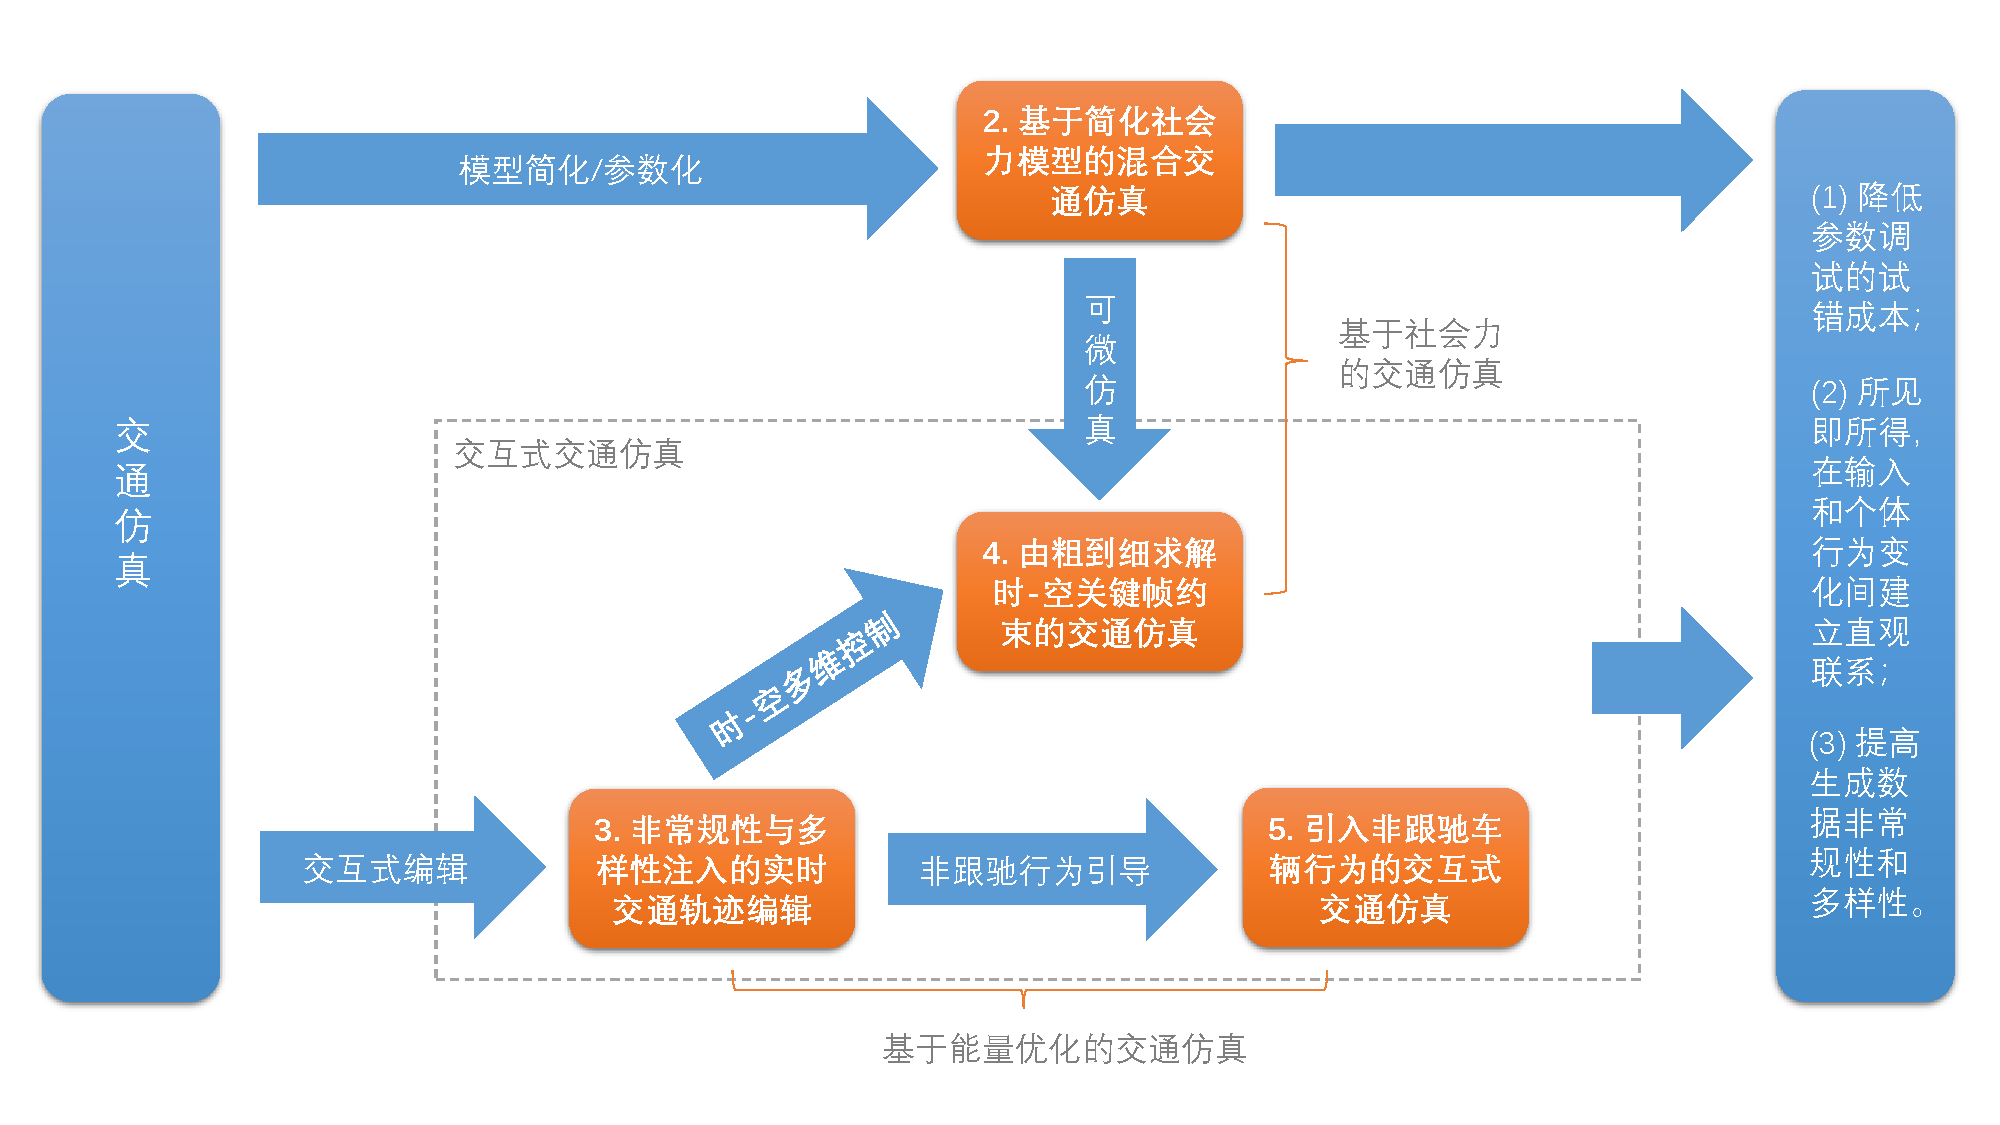
\includegraphics[width=\textwidth]{figure/intro/tot_overview.pdf}
%\caption[本文章节内容之间结构关系示意图]{
%本文章节内容之间结构关系示意图,第2章介绍了基于简化社会力模型的混合交通仿真,第3章介绍了非常规性与多样性注入的实时交通轨迹编辑,第4章介绍了由粗到细求解时-空关键帧约束的交通仿真,第5章介绍了引入非跟驰车辆行为的交互式交通仿真。
%}
%\label{fig:intro_overview}
%\end{figure}


本文后续的章节将在回顾相关工作之后,详细介绍提出的可视化交通仿真运动控制与交互式编辑方法,包括旨在提升智能体行为多样性的交互式交通仿真与轨迹编辑框架、基于时-空关键帧控制的交通仿真、基于用户引导注入非跟驰行为的交通仿真,和旨在提升智能体种类多样性的基于简化社会力模型的混合交通仿真,各工作之间的关系如图~\ref{fig:intro_overview}。本文后续的详细内容如下:

\begin{figure}[!htb]
\centering
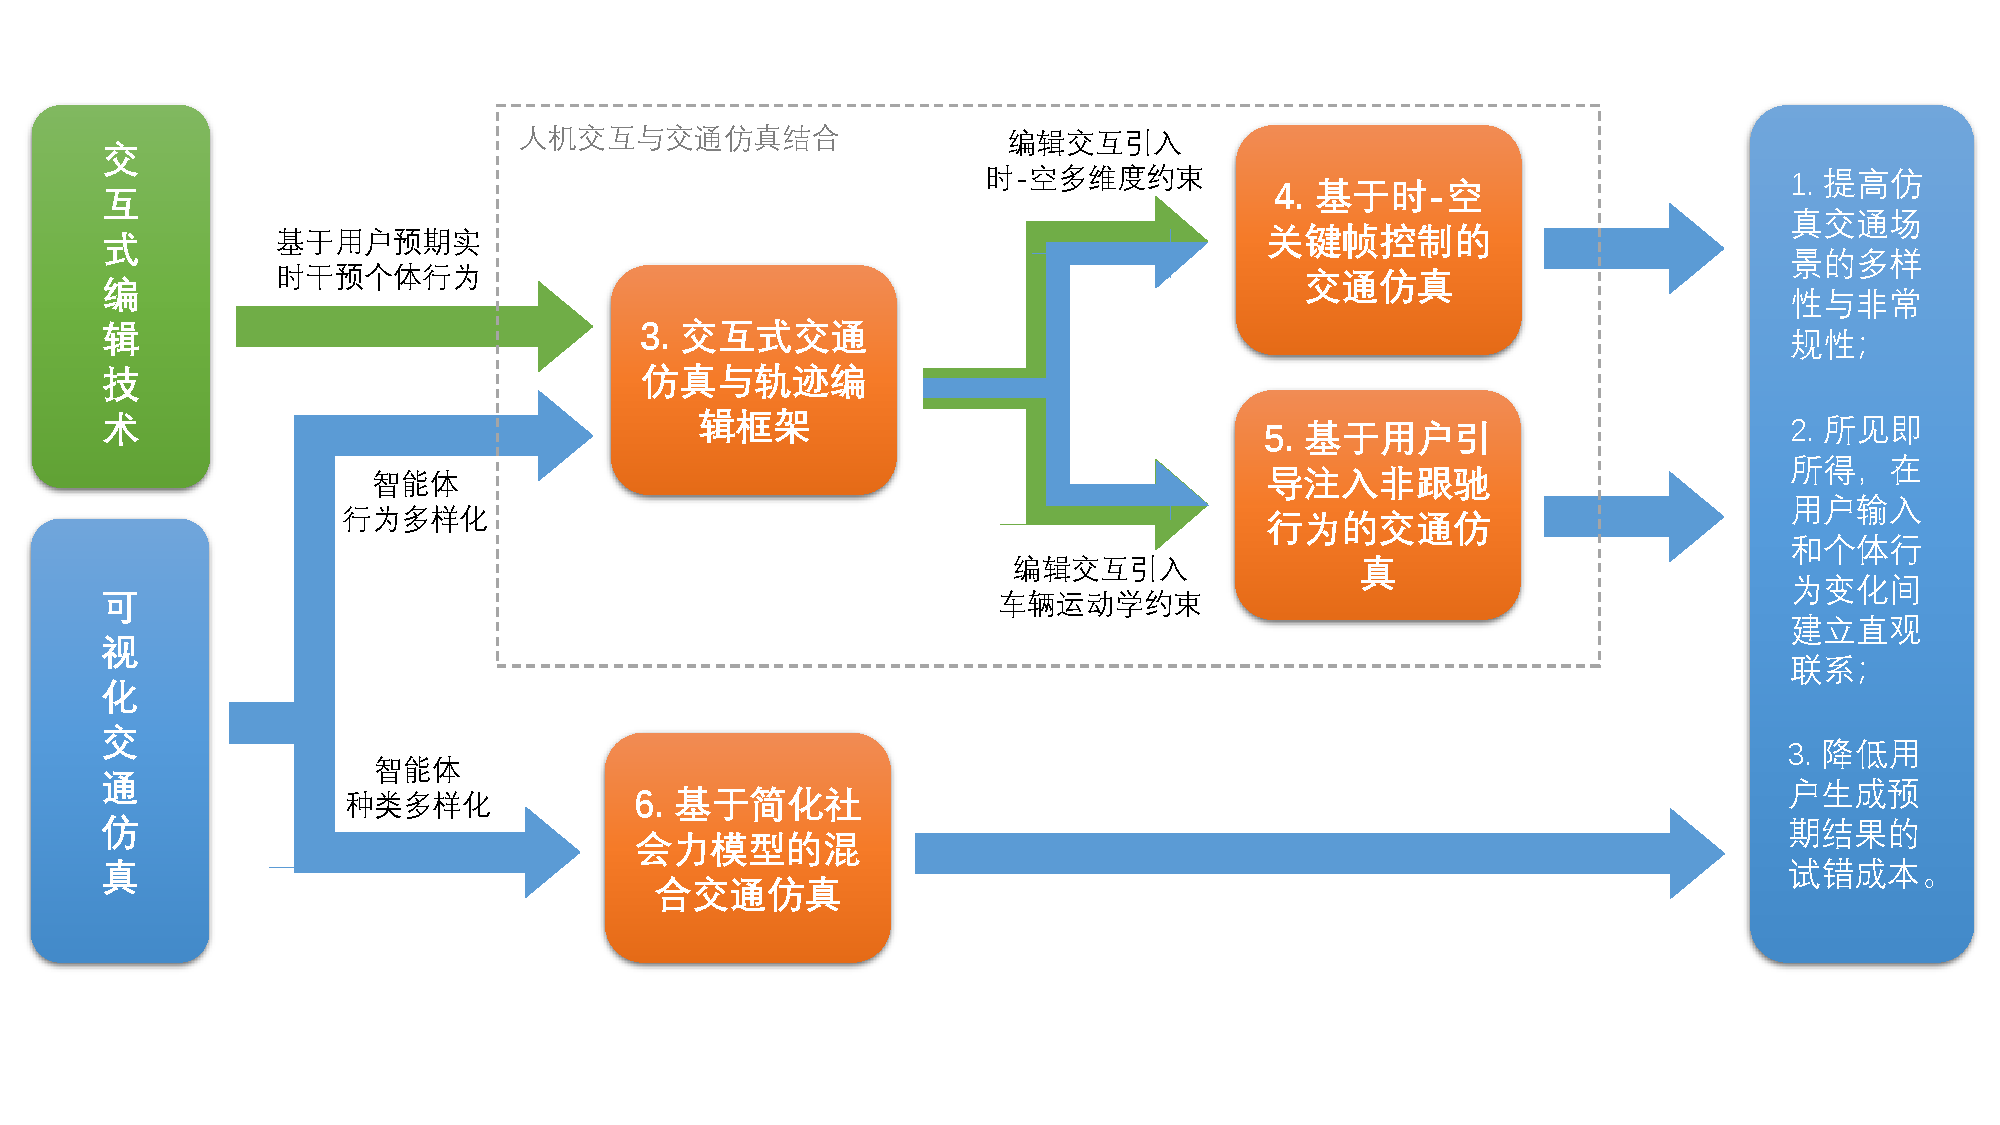
\includegraphics[width=\textwidth]{figure/intro/tot_overview_v4.pdf}
%\caption[本文章节内容之间结构关系示意图]{
%本文章节内容之间结构关系示意图,第2章介绍了基于简化社会力模型的混合交通仿真,第3章介绍了非常规性与多样性注入的实时交通轨迹编辑,第4章介绍了由粗到细求解时-空关键帧约束的交通仿真,第5章介绍了引入非跟驰车辆行为的交互式交通仿真。
%}
\caption[本文章节内容之间结构关系示意图]{
本文章节内容之间结构关系示意图
}
\label{fig:intro_overview}
\end{figure}

在第2章中,我们将详细介绍各个领域的研究现状:首先会针对群组动画中的运动控制技术进行回顾,然后介绍交通仿真中所使用的车辆运动学建模和驱动模型类型,最后对目前交互式编辑技术流行的应用领域和编辑方式分别进行介绍。%在介绍了相关技术的研究现状后,我们也会明晰本文的主要研究内容和后续的行文结构。

在第3章中,为了提高交通仿真中智能体行为的多样性,同时让用户定制化生成包含预定车辆行为的轨迹数据,我们提出了一个非常规性与多样性注入的实时交通轨迹编辑框架。在框架中的交通仿真模块里,车辆的状态同时在欧式坐标系和非欧坐标系中表示,且基于真实数据驱动来更新车辆运动,使其从严格在车道中心处行驶变为跟随参考路径行驶,表现出更灵活且多样的行为。在框架中的全局规划模块里,仿真的场景被离散化为二维的网格平面,车道几何信息使用胶囊状近似来存储到网格中,用户可以使用指定的关键点位置映射到网格单元,基于这些位置通过使用启发式搜索算法来规划新的参考路径。本方法能够快速生成满足用户预期的交通轨迹,且能够生成如U型掉头、急转弯和借道超车等原先方法或数据集中不常见的行为。

在第4章中,为了提高用户交互式轨迹编辑的灵活性,我们将关键帧引入交通仿真动画中,基于用户指定关键帧来生成满足其时-空约束的车辆运动轨迹。相似地,我们在仿真阶段同样将车辆的状态同时使用沿着参考路径坐标和全局坐标表示,且为了满足后续求解关键帧约束的需求,我们提出了一个新颖的可微社会力交通仿真模型。在用户对某辆车辆指定关键帧后,我们设计了一个由粗到细求解约束的优化过程:首先,在沿着参考路径方向上的离散化车辆状态-时间空间内构建状态迁移的有向图,使用启发式搜索算法寻找一条粗略满足关键帧约束的路径。其次,使用粗粒度轨迹中提取的信息来初始化伴随法,使伴随法中的梯度下降过程快速且稳定的收敛,而不会因为初始值选取的不佳导致优化过程的发散。最终,我们得到了一条满足时-空约束且非常平滑的车辆运动轨迹。

在第5章中,为了突破传统交通仿真方法大多基于跟驰模型的约束,我们提出了一种利用用户输入信息来引入倒车行为,从而生成包含非跟驰运动的轨迹的交互式交通仿真方法,从而让用户获得在自定义的“如果”情况下车辆可能采取的行为。我们提出了使用关键状态来同时表征车辆未来运动的位置和朝向信息,并在基于车辆运动学生成的连续空间中使用启发式路径规划方法,生成同时包含前向和反向导航的参考路径。为了调整车辆沿着自定义参考路径的运动和邻车的反馈,我们在速度空间中基于采样和能量最优化策略来更新车辆的运动。特别地,对于车辆之间的相互影响,我们在碰撞避免能量项中同时考虑了安全跟随距离的软约束和车辆几何的边界硬约束;并且使用特别定义的车辆交互规则以明细不同运动类型车辆之间的避让优先级,防止因互不相让引起的交通瘫痪。本方法能快捷生成包含非跟驰运动的交通场景,且让倒车运动的车辆和其邻车对其的反馈更平滑、真实。

在第6章中,为了在统一框架内仿真不同类型的智能体,提高交通仿真中智能体种类的多样性,同时避免大量无实际物理意义且ad-hoc的可调模型参数,本文提出了一种基于简化社会力模型的混合交通仿真方法。基于面向对象的思想,我们设计了一个用于表达不同种类智能体之间运动共性的基类,并通过分析之前的方法所用的社会力模型趋势,设计了一个简化的模型用于计算个体相互影响的各类吸引力和排斥力。利用不同个体拥有的不同物理属性,我们进一步把基类中的系数参数化,使基类派生得到不同的智能体,不仅实现了智能体种类的多态,也实现了相同种类不同个体行为的个性化。

在第7章中,我们总结了本文提出的多种交通仿真与交互式轨迹编辑技术,回顾了各个部分的主要思想和创新之处,并简要探讨了有价值的改进和探索方向。

另外,本文后续中所有涉及交通仿真的描述,若无特别说明,均指代可视化交通仿真技术。



\chapter{相关工作介绍}

%\section{群组动画的发展}

\section{群组动画与运动控制}
\label{section:intro_crowdcontrol}

\subsection{发展与应用}

最初,Reynolds等人~\cite{reynolds1987flocks}提出了基于群体协作的运动控制方法用于模拟鸟群的飞翔模式,研究鸟群行为中的集体动态和自组织特性,而该方法也被视为群组动画领域的开创性工作。随后,群组动画结合不同的约束建模,被广泛被应用于各类生物群体的行为模拟展示,如基于深度学习的方式来建模鱼群运动随日出日落和洋流的影响~\cite{ishiwaka2021foids, ishiwaka2022deepfoids},基于特定的信息传递策略在鸟群飞行~\cite{ren2018stable}或蚂蚁觅食~\cite{xiang2019biologically}时实现个体之间的信息共享,基于仿生学在蝴蝶群体的运动控制中引入骨骼动画~\cite{chen2022practical}以提升呈现结果的视觉真实感等等。人作为高等动物,研究者们在研究人的运动控制时,会尝试对人的心理、生理、社会等因素进行建模,例如人群在火灾等危险环境中的恐慌程度~\cite{helbing1995social}和体力因素~\cite{xu2020emotion}对行为模式的影响。

而车辆作为驾驶载具,汽车的运动可以看做是由人控制的智能体的运动,因此车流的运动也可以作为群组动画的一种特殊类型~\cite{wang2017survey},借鉴群组动画中运动控制的思路,并通过在个体运动控制策略中融合车辆特有的各类约束来展开研究~\cite{herman1963vehicular, reynolds1999steering}。作为群组动画中两个常用的运动控制技术,路径规划和碰撞避免主要用于生成目标驱动和交互避让的行为。本质上,碰撞避免是路径规划过程中经常考虑的一个约束,因此路径规划和碰撞避免通常协同工作,以实现个体在环境中安全、高效的移动。而作为本文主要涉及的运动控制方法,接下来我们将对其分别进行介绍。


\subsection{路径规划}

路径规划是指为移动体(例如机器人、无人机、车辆等)在给定环境中找到一条合适的路径,以使其从起始点到达目标点,并避开障碍物或遵循特定的约束条件,其在许多领域中都有广泛的应用,如自动驾驶车辆、无人机航迹规划、机器人导航、游戏AI等。路径规划的主要过程通常包括对环境的建模表示、路径搜索以及路径后处理优化。

\textbf{地图表示:}地图表示是路径规划中的第一个步骤,用于将环境转换为计算机可处理的形式,方便后续的路径搜索。最简单的表示方法是将场景离散化为栅格地图,其将环境根据任务划分为规则的矩形网格,并使用离散值、向量、势能等表示网格的状态,以区分障碍物、自由空间~\cite{lee2011smooth, lee2013hierarchical},或生成方向场~\cite{sakuma2005psychological, patil2010directing}等。但由于网格大小由离散化分辨率确定,较大的网格可以降低计算复杂度,但会损失细节和准确性,且不同尺寸、几何的障碍物等场景信息很难用规则的矩形准确地逼近。因此,为了解决使用栅格地图表示场景的确存在的精度上的限制,研究者们提出了使用三角网格~\cite{lamarche2004crowd, kallmann2005path}、Voronoi图~\cite{choset1996sensor, sud2007surface, sud2008real}等更灵活的地图表示方法,根据特定的规则将场景划分为若干复杂形状的区域,使环境特征能更精确地编码进存储数据结构中。此外,由于使用传感器采集行车数据的技术越发成熟,也出现了许多直接使用激光雷达点云数据~\cite{chen2015safe}或是基于采集数据构建隐式曲面~\cite{breitenmoser2012surface}来表征场景的方法,进一步提供丰富的三维结构信息或具有连续性的几何信息。

\begin{algorithm}[!b]
\setstretch{1.45}
%\setlength{\abovecaptionskip}{-0.05cm} 
%\setlength{\belowdisplayskip}{-0.25cm}
\caption{A*算法}
\label{alg:intro_Astar}
\begin{algorithmic}[1]
%\Procedure{A*}{$start, goal$}
    \STATE 初始化开集合$O$为空;  %\Comment{O list}
    \STATE 初始化闭集合$C$为空;  %\Comment{C list}
    \STATE 将起始节点 $start$ 加入开集合 $O$
    \WHILE{$O$ 不为空}
        \STATE $current \gets$ 在开集合$O$中启发值$f$最小的节点;  %\Comment{Select node with lowest $f$ score}
        \STATE 将节点$current$从开集合$O$中移除;
        \STATE 将节点$current$加入闭集合$C$;
        \IF{当前节点$current$为目标节点$goal$}  %\Comment{Path found}
            \STATE \textbf{return} 从节点$start$到$current$的路径;
        \ENDIF
        \FORALL{节点$current$的相邻节点$neighbor$}
            \IF{节点$neighbor$不可到达 or 节点$neighbor$在闭集合$C$中}
                \STATE \textbf{continue};
            \ENDIF
            \STATE $new\_g \gets g(current) + \text{cost}(current, neighbor)$;  %\Comment{Calculate $g$ score}
            \IF{节点$neighbor$不在开集合$O$中 or $new\_g$ < $g(neighbor)$}
                \STATE 更新 $g(neighbor) \gets new\_g$;
                \STATE 更新 $h(neighbor) \gets$ 启发式函数计算节点; $neighbor$ 到目标节点 $goal$的代价;
                \STATE 更新 $f(neighbor) \gets g(neighbor) + h(neighbor)$;
                \STATE 更新 $parent(neighbor) \gets current$;
                \IF{节点$neighbor$不在开集合$O$中}
                    \STATE 将节点 $neighbor$ 加入开集合 $O$;
                \ENDIF
            \ENDIF
        \ENDFOR
    \ENDWHILE
    \STATE \textbf{return} 路径搜索失败;  %\Comment{No path found}
%\EndProcedure
\end{algorithmic}
\end{algorithm}

% \begin{algorithm}[!tbh]
% \setstretch{1.15}
% %\setlength{\abovecaptionskip}{-0.05cm} 
% %\setlength{\belowdisplayskip}{-0.25cm}
% \caption{A* Algorithm}
% \label{alg:intro_Astar}
% \begin{algorithmic}[1]
% %\Procedure{A*}{$start, goal$}
%     \STATE Initialize an empty open set $O$  %\Comment{O list}
%     \STATE Initialize an empty closed set $C$  %\Comment{C list}
%     \STATE Add $start$ to $O$
%     \WHILE{$O$ is not empty}
%         \STATE $current \gets$ node in $O$ with the lowest $f$ score  %\Comment{Select node with lowest $f$ score}
%         \STATE Remove $current$ from $O$
%         \STATE Add $current$ to $C$
%         \IF{$current$ is the $goal$}  %\Comment{Path found}
%             \STATE \textbf{return} path from $start$ to $current$
%         \ENDIF
%         \FORALL{$neighbor$ of $current$}
%             \IF{$neighbor$ is not traversable or $neighbor$ is in $C$}
%                 \STATE \textbf{continue}
%             \ENDIF
%             \STATE $new\_g \gets g(current) + \text{cost}(current, neighbor)$  %\Comment{Calculate $g$ score}
%             \IF{$neighbor$ is not in $O$ or $new\_g$ < $g(neighbor)$}
%                 \STATE Set $g(neighbor) \gets new\_g$
%                 \STATE Set $h(neighbor) \gets$ heuristic estimate of cost from $neighbor$ to $goal$
%                 \STATE Set $f(neighbor) \gets g(neighbor) + h(neighbor)$
%                 \STATE Set $parent(neighbor) \gets current$
%                 \IF{$neighbor$ is not in $O$}
%                     \STATE Add $neighbor$ to $O$
%                 \ENDIF
%             \ENDIF
%         \ENDFOR
%     \ENDWHILE
%     \STATE \textbf{return} failure  %\Comment{No path found}
% %\EndProcedure
% \end{algorithmic}
% \end{algorithm}

\textbf{路径搜索:} 路径搜索算法是路径规划中的关键组成部分,用于找到起始点到目标点的最佳或合适的路径。而作为人工智能领域一个基础的问题,路径搜索算法经过多年的研究已经发展得非常成熟。Dijkstra算法~\cite{dijkstra1959note}作为最经典的算法之一,由E.W. Dijkstra于1959年提出,被广泛应用于有向图中的最短路径搜索。A*算法~\cite{hart1968formal}是在Dijkstra算法的基础上发展而来的,其同时兼具贪心算法的准确性和Dijkstra算法的效率,是目前最流行的路径搜索算法,在游戏开发中被广泛应用。A*算法的过程如算法~\ref{alg:intro_Astar}所示,从起始节点开始,更新当前节点的子节点的加权值,并选择具有最小加权值的子节点来作为当前节点,重复直到到达目标节点或遍历所有节点。其关键主要在于建立计算任意节点$n$加权值的函数$f(n)=g(n)+h(n)$(也被称为启发函数),其中$g(n)$代表从起始节点到节点$n$的实际代价,$h(n)$表示从节点$n$到目标节点所要耗费的成本估计,它们通常采用欧氏距离计算。当$g(n)$不变时,节点$n$的加权值取决于$h(n)$的大小,因此A*算法的搜索过程总是保持朝着目节点方向。


A*算法主要用于静态环境下的全局搜索。然而,在实际应用中,移动机器人的路径规划需要进一步考虑到环境中的动态信息。于是Stentz等人提出了D*算法~\cite{stentz1994optimal},主要用于机器人的路径探索。D*算法将解空间表示为一系列状态,允许在实时环境中快速地修改和重新规划路径,以适应变化的环境。此外,一些学者还研究了D*算法的变种,例如D*场算法~\cite{ferguson2006using}和Theta*算法~\cite{daniel2010theta, xiao2014improved}。而针对车辆或车型机器人在复杂环境中的路径规划问题,Dolgov等人提出了混合A*算法~\cite{dolgov2008practical},核心思想是在离散的网格地图上执行A*搜索,并将连续空间中的状态与离散空间中的网格进行映射。与传统A*算法不同的是,其利用连续空间中的运动模型,例如车辆的运动学模型,来扩展搜索空间中的节点和评估其可行性,如图~\ref{fig:intro_hybridAstar}所示。该方法被广泛应用在自动驾驶的路径规划问题中~\cite{sedighi2019guided, dang2022improved}。

\begin{figure}[!tbh]
%\setlength{\abovecaptionskip}{-0.1cm} 
%\setlength{\belowcaptionskip}{-0.45cm}
\centering
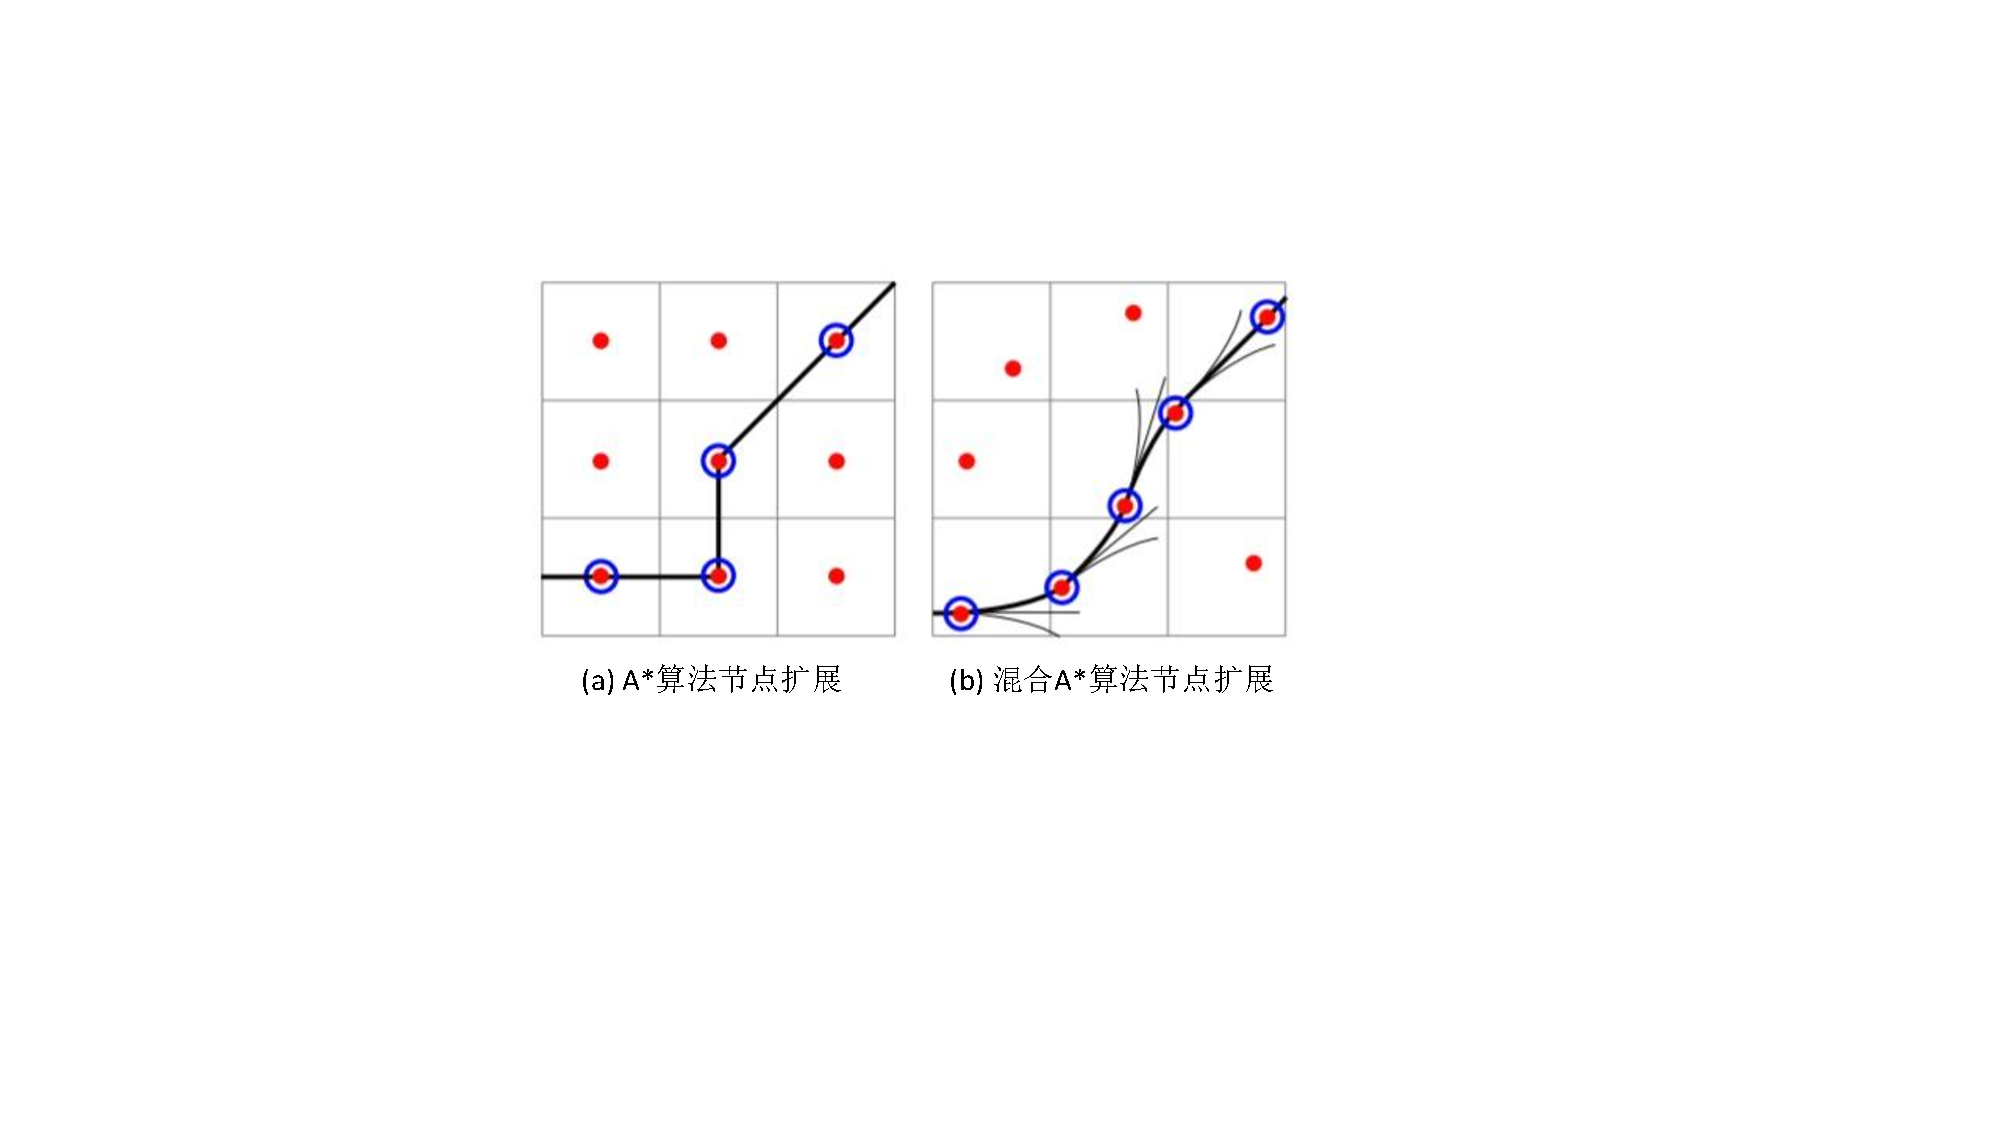
\includegraphics[width=0.7\textwidth]{figure/intro/hybridAstar.pdf}
%\caption[混合A*算法节点扩展示意图]{
%(a) 传统A*算法节点扩展。(b) 混合A*算法基于车辆状态空间与离散网格映射的节点扩展。
%}
\caption[A*算法与混合A*算法节点扩展对比]{
A*算法与混合A*算法节点扩展对比
}
\label{fig:intro_hybridAstar}
\end{figure}


\subsection{碰撞避免}

在群组动画中,碰撞避免算法被广泛应用于模拟和控制多个角色或物体之间的碰撞关系。这些算法旨在确保群组中的个体之间不发生碰撞,同时保持协调和自然的运动。随着自动化技术的不断进步,碰撞避免算法也逐渐成为机器人导航和智能交通领域的重要研究方向。

早年间,群组动画中的碰撞避免一般使用基于群体协作的策略,如经典的Boids算法~\cite{reynolds1987flocks, reynolds1999steering}。该算法通过让角色之间相互观察和响应,根据周围角色的位置和速度来调整自己的运动方向和速度,以保持一定的距离和协调的群体行为。该算法被证实在鸟群、虫群等生物群体的仿真中有着显著的效果。为了更真实地模拟人群的运动,Helbing和Molnar提出了社会力模型(social force model)~\cite{helbing1995social}。他们的模型基于物理学中的力学原理,将人与人之间的相互作用建模为抽象的社会力,考虑了个体的期望速度、社会力和障碍物力,以描述人们在拥挤环境中的运动和互动。随后,社会力模型进行了一系列的扩展和改进。研究者们引入了更多的因素和影响因素,以提高模型的准确性和逼真性。例如,考虑了人们对目标的吸引力、人们对目标的视线范围和注意力、个体之间的互动协作等~\cite{helbing2000simulating, zanlungo2011social, yang2014guided, li2021force}。得益于其实现和计算上的高效,Chao等人也将社会力模型迁移到了混合交通的仿真中~\cite{chao2019force},该方法可以将人、车、自行车等不同种类的交通参与者的运动模拟集成在统一的社会力框架中,并进一步使用真实轨迹数据集对模型中的参数进行标定,减少仿真轨迹与真实轨迹之间的差异~\cite{chao2021calibrated}。而随着机器学习技术的不断成熟,也有许多工作将传统的社会力模型与神经网络相结合,使计算力的参数从大数据中学习得到,最终生成更高质量的仿真结果~\cite{li2019simulation, kreiss2021deep, yue2022human}。


在群体智能领域,速度障碍物(velocity obstacles,简称VO)算法~\cite{fiorini1998motion}是一种考虑了机器人几何信息的碰撞避免算法,主要应用于多机器人系统或移动智能体的协同导航和避障。该算法通过计算速度障碍物域来确定可行的速度范围,以避免与其他移动智能体发生碰撞。针对VO算法中会出现相向而行的两个机器人在避障过程中不断出现抖动的情况,相对速度障碍法(reciprocal velocity obstacles,简称RVO)~\cite{van2008reciprocal}被进一步提出,该算法中除了计算自己的速度障碍物外,还考虑了其他个体对自己的速度的限制,使得在避免碰撞的同时,相对其他个体的速度也要保持在安全范围内。为了进一步适配和优化多个体之间的协同导航和避障,optimal reciprocal collision avoidance(ORCA,也被称为RVO2)算法~\cite{van2011reciprocal}被提出,通过考虑速度的互斥性和相互约束,它能够产生安全、协调的移动智能体轨迹,并能够在实时环境中进行快速的碰撞避免决策,保持很高的运算效率。如图~\ref{fig:intro_orca}(a)所示,假设有两个正在运动中的圆盘状个体A和B,速度障碍$VO^{\tau}_{A|B}$是A相对于B所有会在时间$\tau$内发生碰撞的相对速度集合,定义为:
\begin{equation}
\setlength\abovedisplayskip{10pt}
\setlength\belowdisplayskip{10pt}
\label{eq:intro_orca1}
    VO^{\tau}_{A|B} = \{ \textbf{v} | \exists t \in [0, \tau] :: t\textbf{v} \in D(\textbf{p}_B - \textbf{p}_A, r_A + r_B) \},
\end{equation}
其中$\textbf{p}_A, \textbf{p}_B$是个体A和B的位置,$r_A, r_B$是其圆盘的半径,$D(\textbf{p}_B - \textbf{p}_A, r_A + r_B) \}$代表以点$\textbf{p}_B - \textbf{p}_A$为原点,$r_A+r_B$为半径规划的圆盘区域,通常使用闵可夫斯基和差~\cite{hadwiger1950minkowskische}计算得到,因此如果个体形状并非圆盘时,该区域也会呈不规则多边形。如果此时A相对B的速度会导致A在时间$\tau$内与B发生碰撞,即$\Delta\textbf{v}=\textbf{v}_A - \textbf{v}_B \in VO^{\tau}_{A|B}$,则假设存在向量$\textbf{u}$使$\Delta\textbf{v}$移动最小的距离到达$VO^{\tau}_{A|B}$的边界上,即:
\begin{equation}
\setlength\abovedisplayskip{10pt}
\setlength\belowdisplayskip{10pt}
\label{eq:intro_orca2}
    \textbf{u} = (\mathop{\arg\min}\limits_{ \textbf{v} \in \partial VO^{\tau}_{A|B}} || \textbf{v} - \Delta\textbf{v} || ) - \Delta\textbf{v},
\end{equation}
该式中的$\textbf{v}$在此表示落在$VO^{\tau}_{A|B}$边缘上,使向量$\textbf{u}$长度最小的速度。记向量$\textbf{n}$表示在点$\textbf{u} + \Delta\textbf{v}$指向$VO^{\tau}_{A|B}$外侧的单位向量,则$ORCA^{\tau}_{A|B}$直线可以表示为:
\begin{equation}
\setlength\abovedisplayskip{10pt}
\setlength\belowdisplayskip{10pt}
\label{eq:intro_orca3}
    ORCA^{\tau}_{A|B} = \{ \textbf{v} | (\textbf{v} - (\textbf{v}_A + \frac{1}{2}\textbf{u}))\cdot\textbf{n} \geq 0 \},
\end{equation}
其中$ORCA^{\tau}_{A|B}$直线将个体A的可选速度划分为是否会发生碰撞的两个半平面,如果A在$\textbf{n}$所指的一侧选择速度值更新,就能保证不与个体B碰撞(如图~\ref{fig:intro_orca}(b)所示)。这一思想后续还被拓展到不同形状的车辆或是其他种类交通参与者~\cite{ma2018efficient, luo2022gamma}的碰撞避免计算中,用于轨迹的仿真或预测等任务。

\begin{figure}[!tbh]
%\setlength{\abovecaptionskip}{-0.1cm} 
%\setlength{\belowcaptionskip}{-0.45cm}
\centering
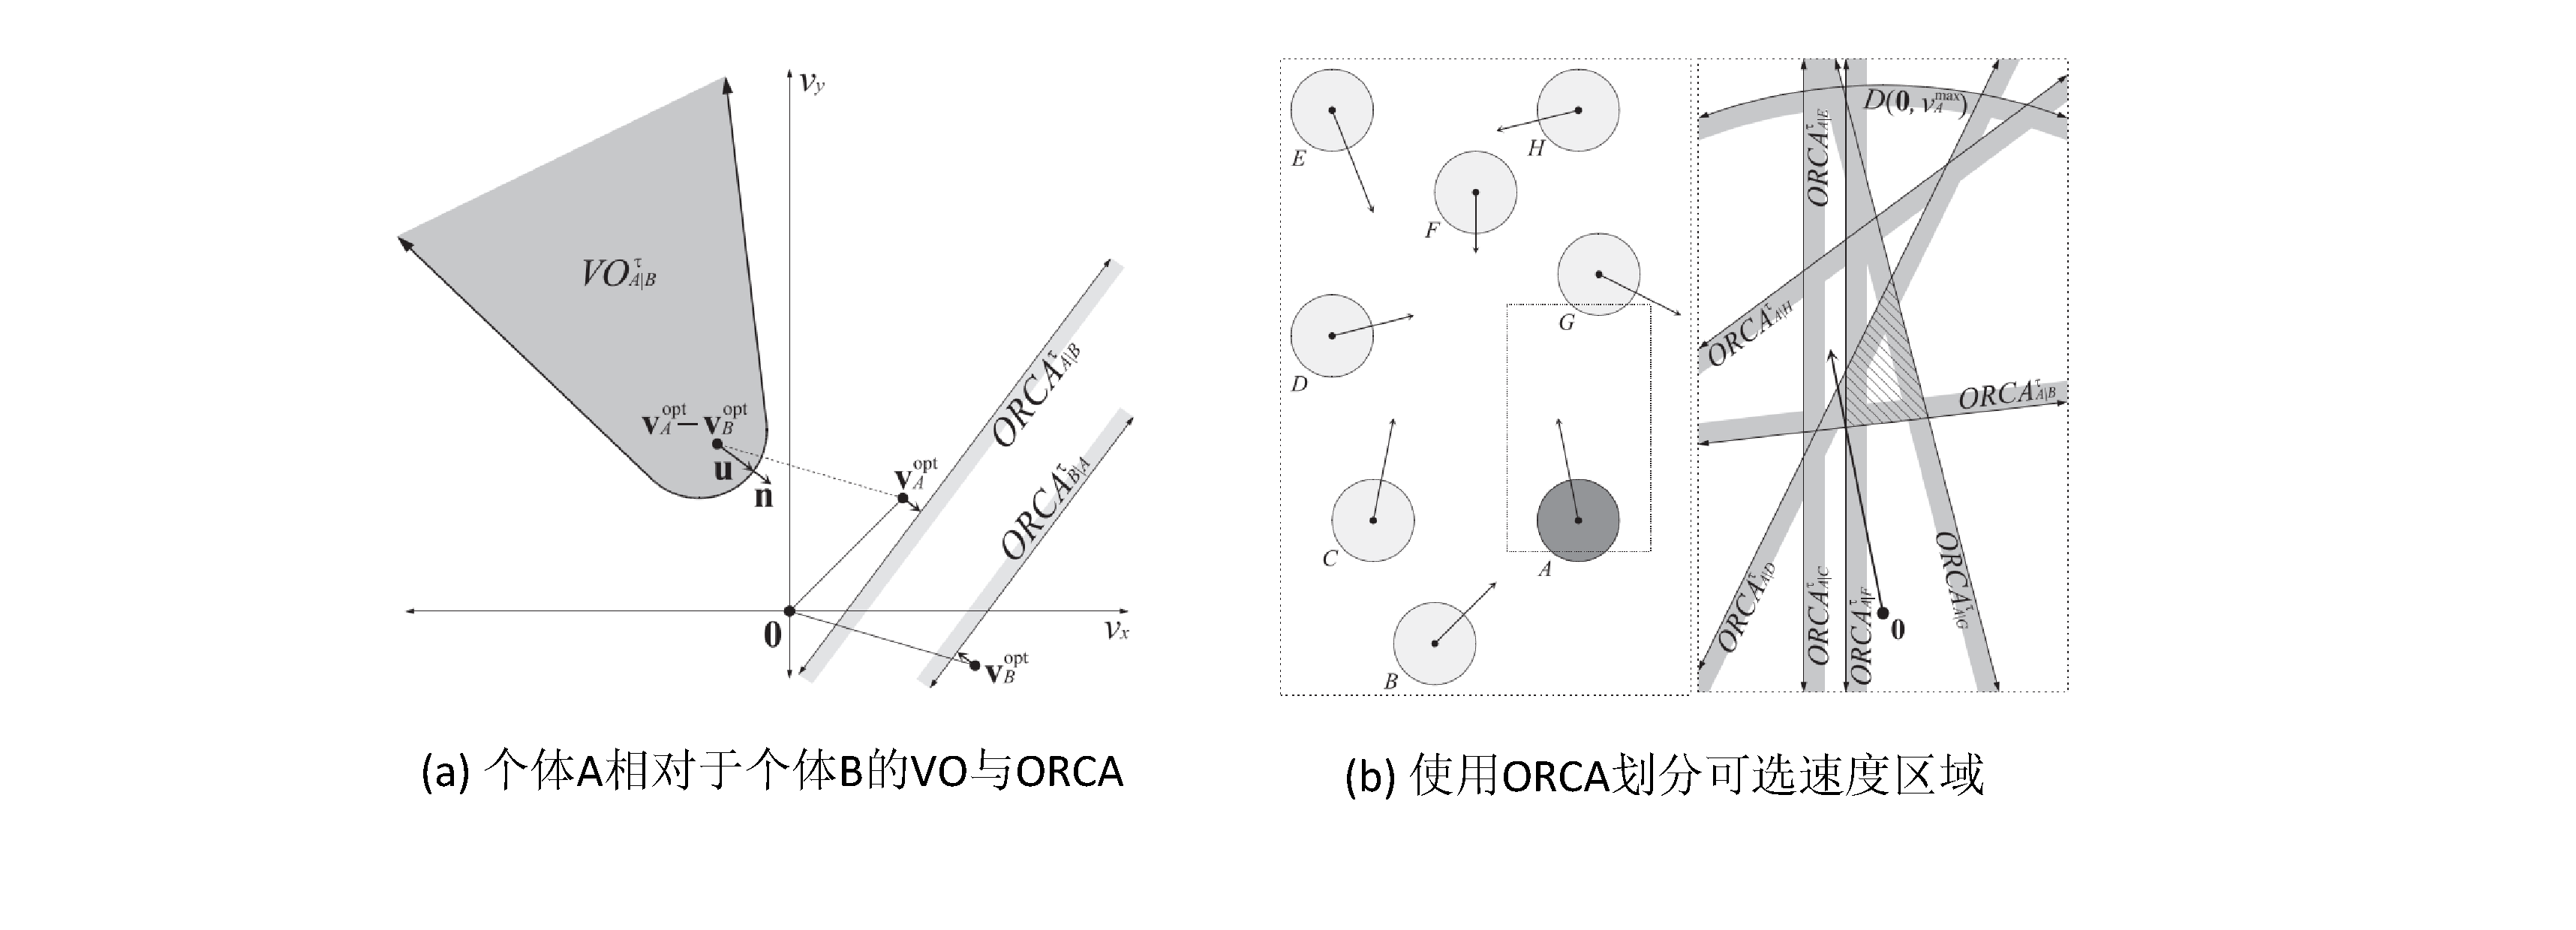
\includegraphics[width=0.93\textwidth]{figure/intro/orca v2.pdf}
%\caption[速度障碍物与ORCA算法示意图]{
%(a) 个体A相对于个体B的速度障碍物(VO)与对应的ORCA。(b) 多智能体运动场景中用ORCA划分可选择速度区域。
%}
\caption[VO与ORCA的计算与应用示意图]{
VO与ORCA的计算与应用示意图
}
\label{fig:intro_orca}
\end{figure}



%接着,Heppner等人~\cite{heppner1990stochastic}也提出了一种随机非线性模型来研究鸟群的协同飞行。随后,群体运动控制被推广到有相似集群行为模式的鱼群~\cite{tu1994artificial, tu1994perceptual}或昆虫群体~\cite{xiang2020fastswarm}中,用于模拟不同物种在环境中的觅食、求偶或逃避天敌等行为。





\section{车辆与交通运动建模}

\label{section:intro_vehiclemove}

与群组动画中的通常模拟的人群、虫群、鸟群等生物群体不同,交通中的车辆运动有其独特且严格的规则限制。首先,车辆的运动必须满足其运动学模型,车辆的加、减速都是过程性的,无法像行人一样能够在任意时刻突然改变朝向和速度,也不能在无前进速度的情况下产生垂直于朝向的横向位移。其次,车辆在标有车道线的道路上行驶时,除了有严格的交通规则要遵守外,还会有一些约定俗成的驾驶习惯,例如时刻安全行车距离等。因此,车辆的运动和交互通常用一套独特的数学和物理模型表示,能更直观地描述车辆在道路上行驶状态的表示方式。


\subsection{车辆运动学}

在控制理论和机器人等领域,非完整系统(non-holonomic system)是一个重要的概念,它描述了系统在特定约束下的运动行为。非完整约束意味着个体对象在某些方面上的运动是受限制的,其自由度小于其物理系统的维度~\cite{ne_mark2004dynamics}。车辆也被称为移动机器人,是一种典型的非完整系统,其非完整约束是车辆无法侧向滑动或横向移动。这意味着车辆实际可运动的方向小于其系统整体可运动的维度,因此车辆的前进方向和转向输入对其最终运动轨迹具有重要影响。


%%https://zhuanlan.zhihu.com/p/443498698
运动学自行车模型(kinematic bicycle model)是一个对非完整系统简化的数学建模,用于描述自行车或是汽车运动过程。它基于运动学原理假设车辆只能在二维平面上移动,但忽略了车辆的动力学和悬挂系统等复杂因素,主要用于模拟预测车辆的运动轨迹,进行路径规划和控制算法的设计~\cite{d1991modelling, kanayama1991stable, kong2015kinematic, polack2017kinematic, freire2022optimal},在车辆自动驾驶领域发挥着重要作用。在如图~\ref{fig:intro_bicycle&frenet}(a)的自行车模型中,假设后轮是车辆的驱动轮,$(x_f, y_f)$和$(x_r, y_r)$分别是前轮与后轮的笛卡尔坐标,$\theta$是车辆笛卡尔坐标系中的车身朝向角,$\delta$是车辆笛卡尔坐标系中的车轮转向角,$\omega$是车轮转向的角速度,$v$是驱动轮赋予车辆沿着车身方向的速度,$L$是车轮轴距长度。则车辆的状态记为$(x, y, \theta, \delta)$,车辆运动的控制输入记为$(v, \omega)$。在车辆无横向移动,即驱动轮赋予车辆垂直于车身方向的速度始终为0的前提下,车辆运动时状态的增量$(\dot{x}, \dot{y}, \dot{\theta}, \dot{\delta})$与控制输入之间的依赖关系可表示为:%车辆在笛卡尔坐标系中的速度可以表示为:
\begin{equation}
\setlength\abovedisplayskip{10pt}
\setlength\belowdisplayskip{10pt}
\begin{aligned}
    \dot{x} &= vcos(\theta), \\
    \dot{y} &= vsin(\theta), \\
    \dot{\theta} &= v\frac{tan(\theta)}{L}, \\
    \dot{\delta} &= \omega,
\end{aligned}
\label{eq:intro_bicycle1}
\end{equation}
其中$\dot{x}, \dot{y}$分别是车辆在笛卡尔坐标系坐标中的速度沿两个坐标轴的分量,$\dot{\theta}$是车辆朝向角的变化速度,$\dot{\delta}$等价于车轮转向的角速度。

\begin{figure}[!tbh]
\centering
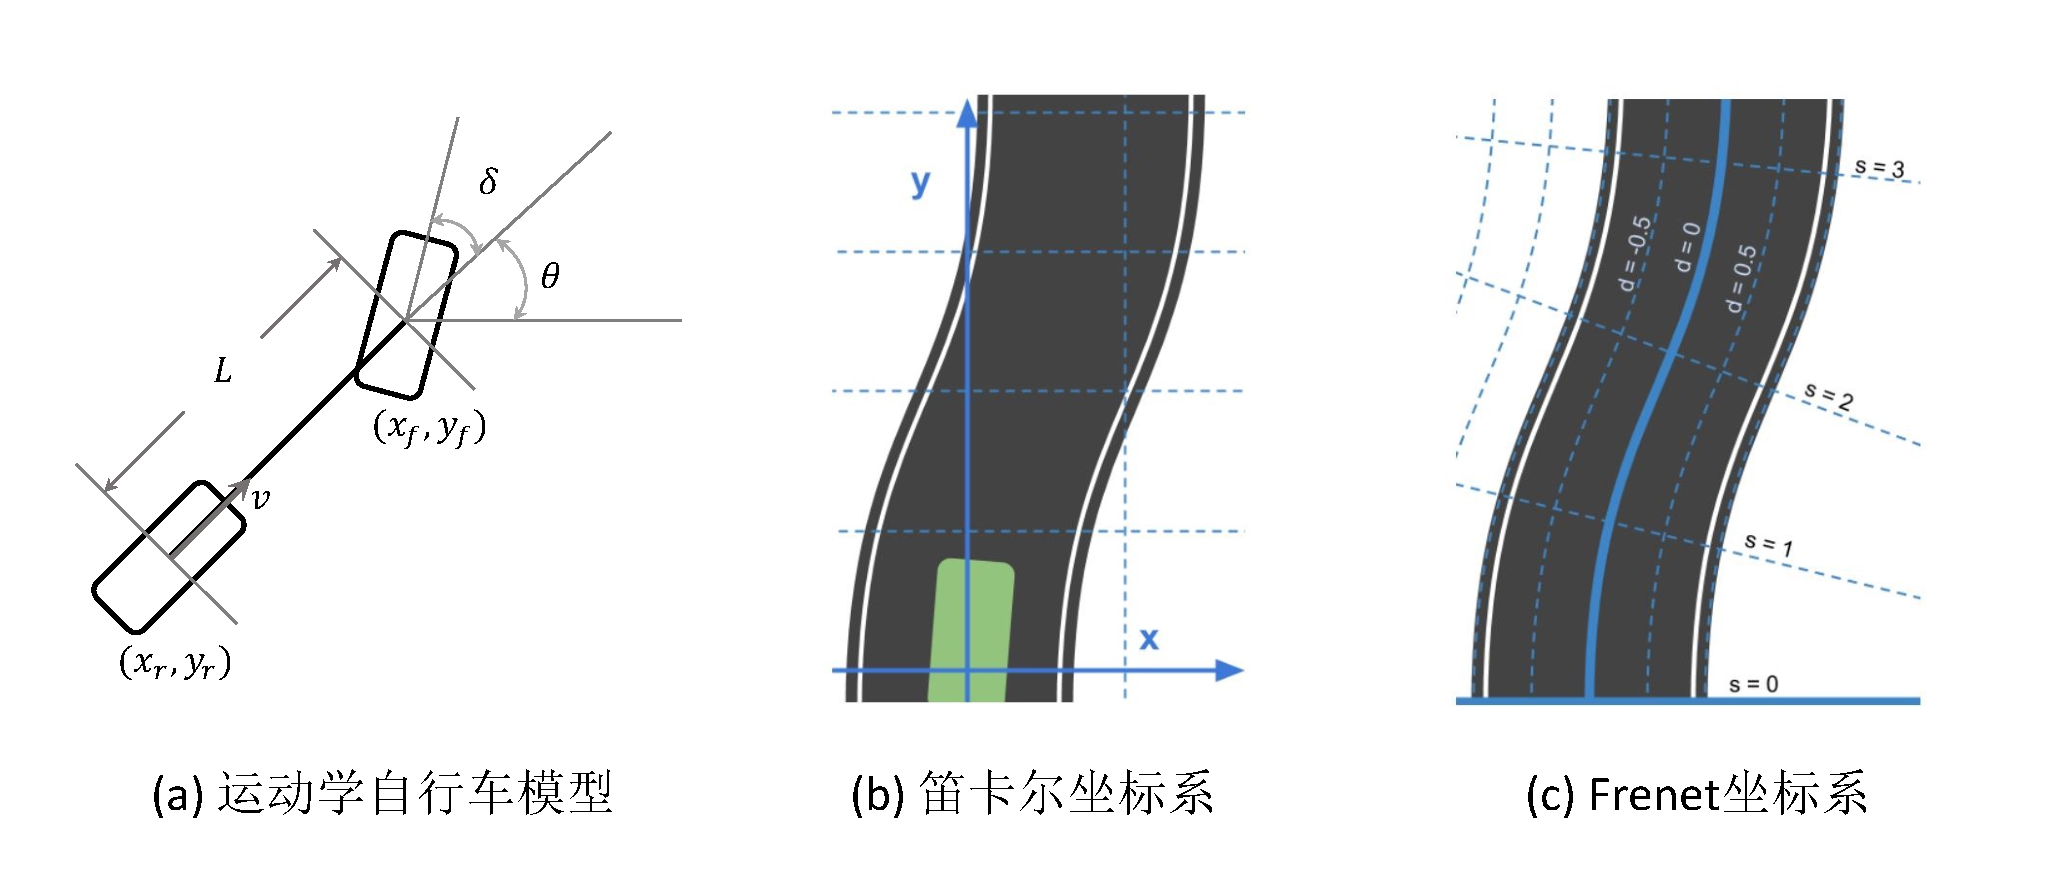
\includegraphics[width=\textwidth]{figure/intro/bicycle & frenet v2.pdf}
%\caption[运动学自行车模型与Frenet坐标系]{
%(a) 运动学自行车模型。(b) 车道与笛卡尔(Cartesian)坐标系。(c) 车道与Frenet坐标系。
%}
\caption[车辆运动学模型与坐标表示]{
车辆运动学模型与坐标表示
}
\label{fig:intro_bicycle&frenet}
\end{figure}

在数学中,笛卡尔坐标系是一种正交坐标系,由两条相互垂直且相交于原点的坐标轴构成。但是对于在道路上行驶的车辆而言,相比于笛卡尔坐标系(图~\ref{fig:intro_bicycle&frenet}(b)),Frenet坐标系提供了一种针对道路几何特征的局部表示方式,可以更好地描述车辆在道路上的位置和运动(图~\ref{fig:intro_bicycle&frenet}(c))。Frenet坐标系最早由法国数学家Jean Frenet于19世纪提出,其使用曲线的切线方向、曲率和挠率来定义曲线上的点~\cite{serret1851quelques, frenet1852courbes}。近年来,Frenet坐标系被广泛应用在机器人运动规划和自动驾驶领域。通过将曲线表示为Frenet坐标系中的函数,可以更方便地进行路径规划和轨迹跟踪,使机器人或自动驾驶车辆在曲线路径上进行平滑、连续且高效的运动~\cite{werling2010optimal, yoshihara2017autonomous, zhu2020trajectory}。在Frenet坐标系中,道路的中心线被定义为纵向参考线,表示车辆从道路起点处沿着道路行驶的纵向距离;切线方向表示车辆偏移参考线的横向距离。通过使用这两个距离,可以将车辆的位置和运动状态转换为Frenet坐标系中的坐标,通常使用符号$(s, d)$表示。



\subsection{交通仿真驱动模型分类}

根据所采用模型粒度,交通仿真可以分为宏观交通仿真和微观交通仿真,它们分别从不同的层面来模拟和分析交通流动的行为和性能:宏观交通仿真关注整体交通流量和交通系统性能,而微观交通仿真则着重于模拟和分析交通系统中个体车辆和行人的行为运动。而根据所采取的不同策略和方法,交通仿真又可以分为基于规则的交通仿真和数据驱动的交通仿真:基于规则的仿真可以提供较好的可控性和可解释性,适用于模拟常规的交通情景和进行交通系统的规划和优化;数据驱动的仿真可以利用大量的实际采集的数据来提高仿真的真实性和准确性,能够模拟更复杂的交通行为和预测交通流动的变化。

\textbf{宏观交通仿真:} 宏观交通仿真(macroscopic traffic simulation)是研究交通系统整体行为和交通流动态的一种仿真方法。在宏观仿真中,交通流量被描述为一个连续的流动,而不是单个车辆或行人的行为。宏观仿真通过定义车流密度、速度和流量等因素之间的关系,来模拟和预测整个交通网络中的交通流动情况~\cite{wang2017survey, chao2020survey}。

LWR模型~\cite{lighthill1955kinematic}是最早用于描述交通流动的宏观模型之一,最初由Lighthill和Whitham提出,之后由Richards进行了扩展。该模型将交通流看作是车辆密度和流量的函数,并通过守恒方程来描述交通流的变化。对交通流的非线性跟随模型的扩展和改进后,GHR模型~\cite{gazis1961nonlinear}应运而生,其核心思想是假设车辆的行为是通过观察和响应前车的运动而产生的,即车辆会模仿前车的速度和加速度来调整自己的行驶状态。为了模拟除了拥堵和自由流以外更复杂的交通情况,PW模型~\cite{payne1971model, whitham1974linear}作为第一个高阶模型,进一步引入了动量守恒方程。随后,CTM模型~\cite{daganzo1994cell}又对LWR模型进行了改进,将道路划分为若干个离散的单元格,每个单元格表示一个道路段或交通区域,通过定义进出车辆的流量来描述交通流动,相较于LWR模型考虑了车辆的加速度和减速度,可以更准确地模拟交通流的变化。而基于PW模型,ARZ模型~\cite{aw2000resurrection, zhang2002non}使用多种方法分别推导出了车流中车辆速度的梯度模型,更精确地对车流中的各向异性进行建模。在计算机图形学领域,Sewall等人~\cite{sewall2010continuum}首次提出了基于宏观流体模型的三维交通流仿真方法,该方法引入了变道的策略将ARZ模型从单车道模型扩展为多车道模型,可以模拟大规模且复杂的城市交通场景,并进行足够真实的三维可视化。

%基于宏观交通仿真模型,目前有如TRANSIMS~\cite{smith1995transims}、AIMSUN~\cite{barcelo2005aimsun}、VISUM~\cite{jacyna2017visum}等仿真系统。利用这些宏观交通仿真系统,研究者们可以评估不同交通规划方案的效果,并找到最佳的交通网络布局、信号灯布局和道路规划,或通过仿真模拟不同的交通控制策略,如交通限制、信号配时~\cite{teklu2007signals}等,最终以提高交通系统的运行效率和交通流的稳定性,减少城市道路拥堵。


\textbf{微观交通仿真:} 微观交通仿真(microscopic traffic simulation)相比于宏观方法更适合研究个体行为和交通流动的细节。在微观仿真中,每辆车或行人都有自己的属性和行为规则。例如,车辆可能根据路口信号、车速限制和周围车辆的位置来做出加速、减速和转向的决策;行人可能会根据行人交通规则、信号灯和周围环境来决定其行走路径和速度。

微观仿真模型通常可分为元胞自动机或跟驰模型~\cite{saifuzzaman2014incorporating, wang2017survey, chao2020survey}。基于元胞自动机,道路网络划分为离散的元胞,代表道路上的一个特定位置,并具有一定的状态和规则,而车辆的运动被建模为移动的元胞~\cite{nagel1992cellular, knospe2004empirical}。得益于简单的实现,这类方法可以应用于大规模道路网络的仿真,但由于离散的性质,其也缺乏对复杂交通行为的精细化表征能力。基于早年的交通仿真工作~\cite{pipes1953operational, herman1963vehicular},Gipps等人最先明确提出了车辆的跟驰模型(car-following model),用于描述车辆在道路上的行驶和跟随行为~\cite{gipps1981behavioural}。该模型基于车辆的速度和距离,通过定义加速度和减速度函数来模拟车辆的行驶行为。在此基础上,最优速度模型(optimal velocity model)被提出并用于对交通拥堵场景的行为建模和数值分析~\cite{bando1995dynamical},而智能驾驶员模型(intelligent driver model,简称IDM模型)则通过额外考虑期望车速和期望车距等因素来进一步优化车辆运动~\cite{treiber2000congested-idm}。

IDM模型因其良好的表现被普遍应用于各类交通仿真器或研究软件中,其由Treiber,Helbing和Kesting等人总结得出,核心思想是车辆的瞬时加速度很大程度上仅由其当前的行驶速度和前车的当前状态所决定,因此只需要少量的参数就能够拟合出逼真的交通流数据。IDM模型的计算表达式如下:
\begin{equation}
\setlength\abovedisplayskip{10pt}
\setlength\belowdisplayskip{10pt}
\label{eq:intro_idm}
    \frac{dv}{dt} = a \left[ 1 - \left(\frac{v}{v_0} \right)^\delta - \left( \frac{s^*}{s} \right) \right],
\end{equation}
其中$\frac{dv}{dt}$表示仿真中车辆的加速度,$a$是最大加速度,$v$是当前行驶速度,$v_0$是预期速度,$\delta$是当前速度与预期速度差值参数,通常取值为4,$s^*$是与前车的预期车距,$s$是与前车的当前车距。模型中的第一项$\left(\frac{v}{v_0} \right)^\delta$为速度差项,当车速越接近期望速度时,速度差项趋近于0,车辆趋向于保持当前速度;当车速不等于预期速度时,速度差项会引起车辆的加速或减速行为。模型中的第二项$\left( \frac{s^*}{s} \right)$表示车距项,当当前车距小于期望车距时,车距项趋近于无穷大,车辆会迅速减速以保持安全距离;当当前车距大于期望车距时,车距项趋近于0,车辆可以保持当前速度或加速。预期车距$s^*$计算表达式为如下:
\begin{equation}
\setlength\abovedisplayskip{10pt}
\setlength\belowdisplayskip{10pt}
\label{eq:intro_idm2}
    s^* = s_0 + vT + \frac{v\Delta{v}}{2\sqrt{ab}},
\end{equation}
其中$s_0$表示最小的安全跟车距离,$T$是安全车头时距,部分工作中也称为制动反应时间,$\Delta{v}$表示车辆与前车的速度差,$b$是期望的最大减速度。


为了进一步提高车辆运动的真实性和多样性,车道变更模型被提出用于描述车辆在多车道道路上的变道行为。MITSIM模型~\cite{yang1996mitsim}考虑了车辆的速度、车距、加速度等因素,并使用概率函数来模拟车辆选择变道的行为,MOBIL模型~\cite{kesting2007general}通过比较变道车辆的边际收益和其他车辆的损失来决定变道行为是否发生。Shen等人将连续变道模型与IDM模型相结合,通过对驾驶员变道意图、环境的参数化分析和变道行为的安全性评估,实现大规模城市路网中车辆的跟驰和变道行为~\cite{shen2012detailed}。此外,通过引入记忆效应来扩展IDM模型可以描述死机对拥挤交通环境的适应性~\cite{treiber2003memory}。而通过对IDM模型与宏观交通流结合的仿真过程进行联合求导,可以进一步提出整体可微的交通仿真模型~\cite{son2022differentiable},为使用数值优化求解仿真中的约束提供了有效的保障。



%目前常用的微观交通仿真系统有如Vissim~\cite{fellendorf1994vissim}、SUMO~\cite{krajzewicz2002sumo}、SimMobility~\cite{adnan2016simmobility}、Carla~\cite{dosovitskiy2017carla}等,利用这些平台可以模拟不同的交通情景和交通规则,并提供对交通流行为和交通控制策略的可视化和分析功能,让用户和研究者们更直观、沉浸地感受真实的交通场景。

\textbf{基于规则的交通仿真:} 基于规则的交通仿真通过定义一系列交通规则和行为模型来模拟交通系统中的车辆和行人的运动。该分类涵盖了绝大多数传统的交通仿真模型,前述讨论过的宏观交通仿真方法和微观交通仿真方法均可归类于此。除了可以对车流或车辆的加减速、变道进行建模外,研究者们还尝试将其他影响交通的因素给融入到交通仿真模型中。通过在仿真场景中添加不同种类的交通参与者,交通仿真器可以生成更多样的交通场景,例如考虑了过马路的行人~\cite{chao2015vehicle, ning2017destination, ningbo2017simulation, chen2019modelling, wang2018shadow}、自行车~\cite{qu2017modeling},甚至是多种类智能体的同时交互的混合交通仿真~\cite{anvari2015modelling, chao2019force, cai2020summit}。基于交通规则或日常驾驶习惯来制定特殊规则,交通仿真器还可以生成车辆在非常规道路上的运动行为,例如在十字路口~\cite{cunto2007microlevel, 2015An}、环岛~\cite{campari2004cellular}、学校门口~\cite{pang2015school}或多种参与者混合的共享空间~\cite{anvari2015modelling}。通过在仿真的同时对其他因素进行额外的建模和统计,研究者们还可以进行诸如红绿灯控制优化~\cite{shen2011agent, mckenney2013distributed, zhao2018signal}、事故发生率预测~\cite{cunto2007microlevel}、天气影响研究~\cite{chen2019assessing}以及二氧化碳排放量统计~\cite{quaassdorff2016microscale}等等。在基于规则的仿真中,交通规则和行为是通过人为预先设定的规则和模型来决定的,模拟的结果均受到这些规则的约束,因此基于规则的仿真可以提供较好的控制性和可解释性。

\textbf{数据驱动的交通仿真:} 数据驱动的交通仿真是一种利用现有的交通数据进行建模和仿真的方法。虽然基于规则的交通仿真已经能够获得非常平稳的交通流,但真实世界的交通场景远比仿真器中设定的要复杂,大量影响交通运行的因素也并不都能通过预定义规则来精准建模,因此仿真的轨迹与真实交通轨迹仍存在一定差异。随着大数据和人工智能的快速发展,数据驱动的交通仿真也越发受到人们的青睐。研究者们通过分析和处理大量真实交通数据,可以揭示隐藏在数据背后的交通参与者的行为模式,并用于预测、仿真和优化交通流动态。

利用如GPS等车载传感器采集的时-空交通轨迹数据,研究者们可以通过启发式搜索~\cite{sewall2010virtualized}、统计推演~\cite{wilkie2013flow}和元模型优化~\cite{li2017city}等方法来重构街道或城市级别的交通流。在特定如十字路口等特殊路段,研究者们也提出了基于学习的交通仿真和车辆编辑方法用于虚拟现实场景展示~\cite{bi2019deep}。通过使用真实交通轨迹数据对IDM模型中的计算参数进行标定,Chao等人先是提出了一种能够使仿真车辆具有个性化运动模式的方法~\cite{chao2013video},随后将相似的思想利用在社会力驱动的混合交通仿真模型中~\cite{chao2021calibrated},减小了仿真轨迹与真实轨迹之间的差异。基于纹理合成和几何形变的思想,Chao等人还提出了一种使用真实数据在任意车道上填充逼真交通流的方法~\cite{chao2017realistic},该方法可以在复杂如立交桥等道路网络上快捷生成交通流(如图~\ref{fig:intro_example}下方所示)。基于能量最小化的策略,Ren等人提出了Heter-Sim~\cite{ren2019heter},一个数据驱动的多智能体仿真系统,不仅可以用于行人和车辆的单独模拟,还能进行多种类智能体混合的交通场景仿真,后续也被证实能应用在虫群的仿真中~\cite{xiang2020fastswarm}。

得益于神经网络技术近年来在各个领域都创造了突破性的进展,研究者们纷纷尝试通过深度学习技术来仿真逼真的交通流。由前Uber首席科学家Raquel Urtasun率领的团队先后提出了利用深度学习仿真得到车辆不同行为的交通仿真器~\cite{suo2021trafficsim},生成各式各样交通场景的场景生成器~\cite{tan2021scenegen},结合混合现实技术对捕捉场景进行重回放式仿真以测试假如车辆采取不同策略的交通结果~\cite{suo2023mixsim},以及利用神经辐射场渲染自动驾驶场景中的相机和雷达数据~\cite{yang2023unisim},旨在为自动驾驶车辆的性能进行高效且全方面的测试。



\section{交互式编辑技术}

交互式编辑技术是一种允许用户直接参与到编辑和创作过程中的技术,其强调的是用户与系统之间的实时反馈和互动。它通过交互式界面和工具,将用户的输入和操作转化为实时的可视化效果或修改结果,使用户能够直观地看到和感受到其编辑行为的影响。这种实时反馈和互动性使得用户能够迅速调整和修改创作内容,从而更好地表达自己的想法和创意。如~\ref{section:intro_challenge}中所述,流畅且直观的交互方式是保证个体行为真实性和仿真运行效率,同时又提高个体行为多样性和用户使用体验的方法,因此本文尝试将这一人在回环(human-in-the-loop)的形式融入到可视化交通仿真中。


\subsection{交互式编辑与内容生成}
% 图像编辑, 艺术作品合成, 室内三维场景生成, 人群动画

交互式编辑技术的目标是提供直观、高效和灵活的编辑体验,使用户能够以自由和创造性的方式进行编辑和创作。它通常结合了图形界面、多点触控、手势识别、实时渲染、物理模拟等技术,以实现用户与编辑系统之间的无缝交互和即时反馈。

交互式编辑技术在图像编辑中提供了直观且灵活的工具,使用户能够对图像进行快速、准确的编辑和修改。例如,交互式选择工具允许用户通过拖拽、绘制或者轮廓跟踪来选择图像中的对象或区域,并进行纹理编辑、图像合成或修改等,大大提升了生成结果的质量和多样性~\cite{ruhl2015interactive, dai2021edit}。除了自然图像外,交互式编辑技术还被应用在艺术品创作领域,艺术家们可以交互式地调整参数、添加特效、处理内容,使其构思的创意和艺术效果能高效变现~\cite{huang2022caripainter}。对于计算机图形学领域的三维场景生成任务,MageAdd~\cite{zhang2021mageadd}被提出用于根据用户偏好交互式地在室内场景中放置合适的物体。该方法根据在数据集中学习到的放置规律,自动在用户光标指示的位置中填充合适的家具或摆设,让用户以最少的输入生成理想的结果。而在群组动画领域,研究者们提出了使用几何形变来对人群轨迹进行时-空方面的约束,大大提升了动画制作师对人群轨迹的控制,避免了生成匹配场景的大规模人群动画的过程中需要反复试错参数并仿真的繁琐过程~\cite{kim2014interactive, zhang2020crowd};对于个体的运动,研究者也提出了使用手绘草稿线来作为仿真中的个体的行进向导或是障碍物边界,从而灵活直观地控制动画的生成过程~\cite{montana2017sketching}。相似的问题在交通仿真中也被提及,用户在想要生成特殊的交通场景或车辆行为时,都需要通过反复试错来获得预期结果。但如前文所述,车辆运动与人群不同,其拥有独特的运动学模型,且需要严格按照交通规则行驶,因此在人群动画中使用的方法并不能简单地迁移到车辆的控制中来,交互式编辑技术与交通仿真运动控制的结合仍然是一个挑战。


%\subsection{关键帧动画}
\subsection{多维交互编辑操作}
% 关键帧-时空优化,##伴随法##

关键帧动画作为允许用户同时在时-空二维度上进行高效编辑的交互式操作,被广泛应用在离散的时序动画制作流程中。它允许用户在时间轴上设置关键帧,定义物体、角色或运动对象在动画序列中的关键状态和位置,然后由算法自动解算关键帧之间的过渡,从而实现平滑的动画效果,让用户使用尽可能少的输入生成满足需求的完整序列帧动画。

作为最优化控制中的经典算法,伴随法(adjoint method)被大量运用在求解关键帧约束的算法中,例如控制流体模拟~\cite{mcnamara2004fluid}、粒子系统~\cite{wojtan2006keyframe}和弹性物体形变~\cite{li2013interactive}等。为了清晰起见,伴随法的过程2可以从一个一般形式的优化问题出发:%伴随法的基本思想是通过拉格朗日乘子法引入伴随变量,将原本带约束的优化问题转化为不带约束的优化问题,构建一个与原问题相逆序的对偶伴随问题,从而通过求解伴随问题的状态变量,计算目标函数对系统参数的梯度。考虑一个一般形式的优化问题:
\begin{equation}
\setlength\abovedisplayskip{10pt}
\setlength\belowdisplayskip{10pt}
\begin{aligned}
    \min_{x}&f(x), \\
    s.t. \quad &g(x)=0,
\end{aligned}
\label{eq:intro_adjoint1}
\end{equation}
其中,$f(x)$ 是目标函数,$g(x)$ 是约束函数,$x$ 是待优化的变量。伴随法的核心思想是通过引入拉格朗日乘子(也称为伴随变量),构造增广拉格朗日函数,并求解其对于原变量和伴随变量的导数。定义增广拉格朗日函数为:
\begin{equation}
\setlength\abovedisplayskip{10pt}
\setlength\belowdisplayskip{10pt}
    L(x, \lambda) = f(x) + \lambda^T g(x).
\label{eq:intro_adjoint2}
\end{equation}
然后,对增广拉格朗日函数求解其对于$x$和伴随变量$\lambda$的导数:
\begin{equation}
\setlength\abovedisplayskip{10pt}
\setlength\belowdisplayskip{10pt}
\begin{aligned}
    \frac{\partial L}{\partial x} &= \frac{\partial f}{\partial x} + \frac{\partial g}{\partial x} \lambda, \\
    \frac{\partial L}{\partial \lambda} &= g(x).
\end{aligned}
\label{eq:intro_adjoint3}
\end{equation}
通过求解伴随方程$g(x) = 0$获得伴随变量的值,最终可以得到目标函数的梯度:
\begin{equation}
\setlength\abovedisplayskip{10pt}
\setlength\belowdisplayskip{10pt}
    \frac{\partial f}{\partial x} = - \frac{\partial g}{\partial x}^T \lambda.
\label{eq:intro_adjoint4}
\end{equation}
但由于梯度下降优化过程十分依赖于参数的初始化值选择,即便交通仿真和粒子系统、群组动画具有相似的理论依据,交通的场景和约束方面也更加复杂,当初始值与最优值差距过大时,无法保证梯度最终一定能够收敛。而在先前的交通流重构工作中,研究者们提出了在车辆的状态-时间离散空间中使用启发式搜索算法能够生成类似于关键帧约束的交通流结果~\cite{van2007kinodynamic, sewall2010virtualized},但由于解空间离散化的粒度太大,最终车辆的运动失真严重。除此之外,由于深度学习的快速发展,数据驱动的关键帧求解、动画补全等,近年来也被大量应用在角色骨骼动画~\cite{xu2018weighted, harvey2020robust, tang2022real}、布料仿真等领域~\cite{wang2019learning}。综上所述,目前鲜有面向交通仿真的关键帧控制求解算法,这极大程度上限制了用户交互式编辑交通仿真轨迹的灵活程度。




